\documentclass[lang=cn,18pt]{elegantbook}

\title{泛函分析}
\subtitle{期末复习讲义}

\author{自不觉}
%\institute{组织}
\date{\today}
\version{2.0}
\bioinfo{更新地址:}{见文档末尾}

\extrainfo{\begin{align*}
    \text{--...-....-...- -.-.---..-.-... ----.--.-..-..- -..--...--..---. -..---.-.-..--. -.-.---..-.-... ----.--.-..-..- -..----.--.....} & \\ 
    & \text{—— Ma DJ}
\end{align*}
 }

\setcounter{tocdepth}{3}

\logo{piclog.jpg}
\cover{01.jpg}

% 本文档命令
\usepackage{array}
\usepackage{extarrows}
\usepackage{latexsym,amsmath,xcolor,multicol,booktabs,calligra}
\usepackage{graphicx,pstricks,listings,stackengine,color}
\usepackage{hyperref}
\usepackage{appendix}

\hypersetup{
    colorlinks=true,
    linkcolor=blue,
    filecolor=blue,      
    urlcolor=blue,
    citecolor=cyan,
}
%改变颜色

\newcommand{\ccr}[1]{\makecell{{\color{#1}\rule{1cm}{1cm}}}}

% 修改标题页的橙色带
\definecolor{customcolor}{RGB}{32,178,170}
\colorlet{coverlinecolor}{customcolor}

\begin{document}

\maketitle
\frontmatter

\tableofcontents

\mainmatter

\chapter{度量空间与赋范线性空间}
\section{度量空间}
\begin{example}
    $[a,b]$上的连续函数空间$C[a,b]$按最大模范数,$\Arrowvert f \Arrowvert=\max\limits_{x \in [a,b]}|f(x)|$构成的度量空间.
\end{example}

\begin{example}
    数列空间按一般范数构成度量空间
\end{example}

\begin{note}
    由于本部分过于简单,故此版本不写入证明过程.关于此类问题,即验证关于某个集合的非负二元函数是否满足度量的性质,此类题一般对于正定性和对称性的证明是显然的,主要在于验证三角不等式是否成立,这需要一些基础的不等式能力,例如绝对值不等式,Cauchy不等式等等,熟练运用不等式放缩即可证明此类问题.
\end{note}

\section{连续函数与连续映射}
\begin{example}
    设$(X,d)$是度量空间,$A \subset X$是闭子集.令
$$f(x)=d(x,A) \xlongequal[]{def}\inf \{d(x,y):y\in A\}$$
证明:$f(x)$是$X$上的连续函数.
\end{example}
\begin{proof}
    $\forall x_{1},x_{2}\in X $,由$d(x,A)$的定义知:$\forall n \in \mathbb{N}^+,\exists y_n \in A\text{有}$
    \begin{align*}
        d(x_{1},A) & \leqslant d(x_{1},y_n)< d(x_{1},A)+\frac{1}{n} \\
        d(x_2,A) & \leqslant d(x_{2},y_n)<d(x_{2},A)+\frac{1}{n}
    \end{align*}

对$\forall n \in \mathbb{N}^+$,由三角不等式可得:
$$d(x_{2},A)\leqslant d(x_2,y_n) \leqslant d(x_{2},x_{1})+d(x_{1},y_n)<d(x_{1},x_{2})+d(x_{1},A)+\frac{1}{n}$$ 
令$n \to +\infty$有$d(x_{2},A)\leqslant d(x_{1},x_{2})+d(x_{1},A) $.从而
$$d(x_{2},A)-d(x_{1},A)\leqslant d(x_{1},x_{2})$$
由$d$的对称性,交换$x_{1},x_{2}$也成立.从而
$$|d(x_{1},A)-d(x_{2},A)|\leqslant d(x_{1},x_{2}) $$\\
$\forall \varepsilon>0,$取$\delta =\varepsilon.$故当$d(x_{1},x_{2})<\delta$时.有$$|f(x_1)-f(x_2)|=|d(x_{1},A)-d(x_{2},A)|<\varepsilon$$  
$\therefore f(x)=d(x,A)$在$X$上一致连续,故连续.
\end{proof}

\begin{note}
    虽然在证明过程中并未用到$A$是闭子集这个条件,但是对于函数$d(x,A)$来说,$A$为闭子集和$A$为非空子集还是有本质区别的,有兴趣请独立思考.
\end{note}

\begin{theorem}
    设$X,Y$是度量空间,则$X$到$Y$的映射$f$是连续映射的充分必要条件是$Y$中任意开集$G$的原像$f^{-1}(G)$是$X$中的开集.
\end{theorem}
\begin{proof}
    必要性:
$f$是连续映射,$G$是$Y$中的开集,若$f^{-1}(G)=\emptyset$,那么$f^{-1}(G)$是开集.若$f^{-1}(G)\not=\emptyset$, 则对 $\forall x_0 \in f^{-1}(G)$, 有 $f(x_0) \in G$. 由于$G$是开集.所以存在$f(x_0)$的$\varepsilon$邻域$B(f(x_0),\varepsilon) \subset G$.由$f$的连续性,则存在$x_0$的$\delta$邻域$B(x_{0},\delta)$,使得$f(B(x_{0},\delta))\subset B(f(x_{0}),\varepsilon)$,即
$$B(x_{0},\delta)\subset f^{-1}(B(f(x_{0}),\varepsilon)) \subset f^{-1}(G)$$
由$x_0$的任意性知$f^{-1}(G)$是开集.

充分性:如果$Y$中每一个开集的原像是开集,对$\forall x_0 \in X,f(x_0)$的任意$\varepsilon$邻域$B(f(x_0),\varepsilon)$的原像$f^{-1}(B(f(x_{0}),\varepsilon))$是$X$中的开集,又$x_{0}\in f^{-1}(B(f(x_{0}),\varepsilon))$,所以$x_0$是内点,因而存在$x_0$的某个邻域$B(x_0,\delta)$.使得
$$B(x_{0},\delta) \subset f^{-1} (B(f(x_{0}),\varepsilon))$$ 

则$f(B(x_{0},\delta)) \subset B(f(x_{0}),\varepsilon)$,即$f$在$x_0$连续,由$x_0$的任意性,$f$是$X$上的连续映射.
\end{proof}




\begin{note}
    将定理中的开集改为闭集,定理仍然成立.
\end{note}

\section{稠密与可分}
\begin{theorem}
    设$E$是可测集,当$1 \leqslant p < \infty$时,$L^p(E)$中的有界可测函数全体$B(E)$是$L^p(E)$的稠密子集.
\end{theorem}
\begin{proof}
    设$f\in L^p(E)$,构造函数列$\{f_n\}$,

    \[
	f_n(x) = 
\begin{cases}
    f(x) &,\quad |f(x)| \leqslant n \\
    0 &,\quad |f(x)|>n
\end{cases}
\]
则$\{f_n\}$是$L^p(E)$中的有界可测函数列,从而$\{f_n\}\subset B(E)$.并且有
$$\int_{E}|f_n -f|^p=\int_{E[|f|>n]}|f|^p$$
由于$|f|^p\in L(E)$,并由积分的全连续性,对$\forall \varepsilon > 0,\exists \delta>0$,使得当$A\subset E,m(A)<\delta$时成立
$$\int_{A}|f|^p<\varepsilon^p$$
由于
$$\int_{E}|f|^p \geqslant\int_{E[|f|>n]}|f|^p \geqslant n^p\cdot m(E[|f|>n])$$
可推出
$$m(E[|f|>n])\leqslant \frac{1}{n^p}\int_{E}|f|^p$$
当$n \to \infty$时,$m(E[|f|>n])\to 0$,故$\exists N$,当$n >N$时,$m(E[|f|>n]) < \delta$.此时有
$$\|f_n-f\|_p=\left(\int_{E}|f_n -f|^p \right)^{\frac{1}{p}}=\left(\int_{E[|f|>n]}|f|^p \right)^{\frac{1}{p}} < \varepsilon. $$
所以$L^{p}(E)$中有界可测函数全体$B(E)$在$L^p(E)$中稠密.
\end{proof}

\begin{theorem}{\textreferencemark Lusin定理}
    令$f$为定义在$E$上的实值可测函数.则对任意$\varepsilon > 0$,存在$\mathbb{R}$上的连续函数$g$和一个包含于$E$的闭集$F$,使得
    $$\text{在}F\text{上}f=g\text{且}m(E-F)< \varepsilon.$$
    
\end{theorem}
\begin{note}
    由于Lusin定理在后文中多次出现,并且此定理在实变函数中具有重要意义,故在此给出Lusin定理的叙述.

    Lusin定理是Littlewood三大原理其中之一,对于一元实变函数论,若能掌握Littlewood三原理,不夸张的说就已经掌握一元实变函数论的大部分内容了.这三个原理可大致表述如下:每个可测集可被区间的有限并逼近;每个可测函数可由连续函数逼近(Lusin定理);每个逐点收敛的可测函数列可由一致收敛的函数列逼近(Egoroff定理).实变函数中大部分结果是这些思想的直观应用.
\end{note}

\begin{theorem}
    当 $1 \leqslant p < \infty$时,$C[a,b]$在$L^p[a,b]$中稠密
\end{theorem}
\begin{proof}
    $\forall f \in L^p[a,b]$,$\forall \varepsilon >0$,由$B[a,b]$在$L^p[a,b]$中稠密,则存在$g \in B[a,b]$,使得$\|f-g\|_p < \frac{\varepsilon}{2}$,不妨设$|g| \leqslant M$,由Lusin定理,对于$\delta=\frac{1}{2^p}\left(\frac{\varepsilon}{2M}\right)^p$,存在$\varphi(x) \in C[a,b]$,使得$m(E[\varphi \not= g]) < \delta$,其中$$E[\varphi \not= g]=\{x \in [a,b]|\varphi(x) \not= g(x)\}.$$

    不妨设$|\varphi| \leqslant M$,否则$\varphi(x)$换成连续函数$\max \{\min\{\varphi(x),M\}-M\}$即可

    则
    \begin{align*}
        \|\varphi -g\|_p=\left(\int_{a}^{b}|\varphi-g|^p\right)^{\frac{1}{p}}& = \left(\int_{E[\varphi \not=g]}|\varphi-g|^p\right)^{\frac{1}{p}} \\
        & \leqslant \left(2^p M^p\cdot m(E[\varphi \not= g]) \right)^{\frac{1}{p}} \\
        & < \frac{\varepsilon}{2}
    \end{align*}
    从而
    $$\|f-\varphi\|_p \leqslant \|f-g\|_p + \|g-\varphi\|_p < \varepsilon$$即$C[a,b]$在$L^p[a,b]$中稠密.
\end{proof}

\begin{remark}
其中
    \[
	\max \{\min\{\varphi(x),M\}-M\} = 
\begin{cases}
    M &, \quad \varphi(x) >M \\
    \varphi(x) &, \quad -M \leqslant \varphi(x) \leqslant M \\
    -M &, \quad \varphi(x) < -M
\end{cases}
\]
\end{remark}
\begin{note}
    在上一命题中,我们知道$B[a,b]$在$L^p[a,b]$中稠密,故此命题只需证明$C[a,b]$在$B[a,b]$中稠密,再由稠密的传递性即可得证.但值得注意的是由于$B(E)$在$L^p(E)$中稠密,度量逼近性质的是$\| \cdot \|_p$,故此,我们在证明$C[a,b]$在$B[a,b]$中稠密时用以度量逼近性质的也应为$\| \cdot \|_p$而不是最大模范数.
\end{note}
\begin{note}
    为了描述赋范空间之间的逼近性质给出以下命题:
    \begin{enumerate}
        \item 限制在$[a,b]$上的多项式族在赋予最大模范数的线性空间$C[a,b]$中稠密;
        \item $E$为可测集,当$ 1\leqslant p \leqslant \infty$时,$L^p(E)$中简单函数构成的子空间在$L^p(E)$中稠密;
        \item 当$1 \leqslant p < \infty$时,$[a,b]$上的阶梯函数构成的子空间在$L^p[a,b]$中稠密;
    \end{enumerate}
    为了得到新的稠密集,我们应该从两个方面出发,一方面我们需要考虑稠密子集的稠密子集,这是因为稠密具有传递性,例如:$[a,b]$上的有理多项式族在多项式族中稠密,自然在$C[a,b]$中稠密.另一方面,我们需要考虑稠密子集的逼近,例如:简单函数可以逼近可测函数,自然的简单函数在可测函数中稠密,由此我们可以通过以上种种命题和各种逼近性质(当然最为著名的逼近结果即为Weierstrass逼近定理,上述命题第一点即Weierstrass第一逼近定理)来构造稠密子集.
\end{note}

\begin{theorem}
    $C[a,b],l^p,L^p[a,b]$是可分的.
\end{theorem}
\begin{proof}
    对于$C[a,b]$和$L^p[a,b]$,由于$P[a,b]$在$C[a,b]$和$L^p[a,b]$中稠密,并且有理多项式$Q[a,b]$在$P[a,b]$中稠密,由稠密的传递性$Q[a,b]$是$C[a,b]$和$L^p[a,b]$的可数稠密子集,从而可分.

    对于$l^p$,令$A_m=\{(r_1,r_2,\cdots,r_m,0,\cdots)|r_i \in \mathbb{Q},i=1,2,\cdots,m\}$,其中$m \in \mathbb{N}^+$,从而$A=\bigcup\limits_{m=1}^{\infty}A_m$是$l^p$的子集,并且可数.

    对$\forall x \in l^p$及$\forall \varepsilon > 0$,由于$\sum\limits_{n=1}^{\infty}|x_n|^p < \infty$,故存在$N$,使得
    $$\sum\limits_{n=N+1}^{\infty}|x_n|^p < \frac{\varepsilon^p}{2}.$$
    由$\mathbb{Q}$在$\mathbb{R}$中稠密,所以对$\forall 1 \leqslant n \leqslant N$,$\exists r_n$,有$|x_n -r_n|^p < \frac{\varepsilon^p}{2^{n+1}}$

    令$y=(r_1,r_2,\cdots,r_N,0,\cdots)$,从而$y \in A$,并且有
    $$\|x-y\|_p=\left(\sum\limits_{n=1}^{N}|x_n -r_n|^p + \sum\limits_{n=N+1}^{\infty}|x_n|^p \right)^{\frac{1}{p}} < \varepsilon.$$
    即$l^p$可分.
\end{proof}


\begin{theorem}
    $l^{\infty},L^{\infty}(E)$不可分.
\end{theorem}
\begin{proof}
    令$M$为$l^{\infty}$中坐标$x_i$取值为$0$或$1$的点$x=(x_1,x_2,\cdots)$全体.则$M$与二进制小数一一对应,所以$M$的基数为$c$.对$M$中任意两个不同点$x,y$,有$d(x,y)=1$,如果$l^{\infty}$可分,则$l^{\infty}$存在可数稠密子集$\{y_i\}$,对$M$中任意一点$x$,作开球$B(x,\frac{1}{3})$,则$\{B(x,\frac{1}{3})|x \in M \}$是一族两两不交的开球,且不可数.由于$\{y_i\}$在$l^{\infty}$中稠密,所以每个$B(x,\frac{1}{3})$中至少含有$\{y_i\}$中一点,与$\{y_i\}$可数矛盾.
\end{proof}
\begin{note}
    从$l^p$不可分的证明中,我们可以看到证明的思路大致是,先找到一个基数为$c$子集$M$,由原度量在其上的限制构成的度量子空间是一个离散度量空间,再假设原空间可分,由稠密的性质,则存在原空间的可数稠密子集到由$M$生成的两两不交的不可数开球族的一个满射,从而可数稠密子集的基数至少为$c$,与可数矛盾.现在我们仿照这个过程来证明$L^{\infty}(E)$不可分,为此我们先证明$L^{\infty}[a,b]$不可分.
\end{note}
\begin{proof}
    令$M$为$L^{\infty}[a,b]$中形如$\chi_{[a,t]},t \in [a,b]$的特征函数全体,则$M$与$[a,b]$的基数对等,为$c$.对$M$中任意两点$\chi_{[a,t_1]},\chi_{[a,t_2]},t_1 \not= t_2$,有$\|\chi_{[a,t_1]}-\chi_{[a,t_2]}\|_{\infty}=1$.如果$L^{\infty}[a,b]$可分,则存在可数稠密子集,记作$\{f_i\}$.对$M$中任意一点作开球$B(\chi_{[a,t]},\frac{1}{3})$,则$\{B(\chi_{[a,t]},\frac{1}{3})|t \in [a,b]\}$是一族两两不交的开球,且不可数.由于$\{f_i\}$在$L^{\infty}[a,b]$中稠密,所以每个$B(\chi_{[a,t]},\frac{1}{3})$中至少含有$\{f_i\}$中一点,与$\{f_i\}$可数矛盾.
\end{proof}
\begin{note}
    在上述证明中我们可以看到对于$L^{\infty}[a,b]$不可分的证明和$l^{\infty}$不可分几乎没有分别.但对于一般的可测集$E$并不一定成立,但是我们有,若$E$是具有正测度的可测集,则$L^{\infty}(E)$不可分.只需将上述$M$替换成$\{\chi_{A}|A \subset E\}$即可.
\end{note}



\section{$L^p$空间中的两个重要不等式}
\begin{theorem}{H$\ddot{\text{o}}$lder不等式}
    设$p > 1.\frac{1}{p}+\frac{1}{q}=1,f \in L^p[a,b],g\in L^q[a,b]$,那么$f(t)g(t)$在$[a,b]$上$L$可积,并且
    $$\int^{b}_{a}|f(t)g(t)|dt \leqslant \Arrowvert f \Arrowvert_p \Arrowvert g \Arrowvert_q$$
\end{theorem}

\begin{proof}
    首先证明Young不等式.即$p > 1,\frac{1}{p}+\frac{1}{q}=1$,对$\forall x,y \geqslant 0$,有
$$xy\leqslant\frac{x^p}{p}+\frac{y^q}{q}$$
若$x,y$中有一个为$0$时,不等式显然成立,下证$x,y>0$,由 
\begin{align*}
    xy=e^{\ln{xy}}=e^{\ln{x} +\ln{y}} & =  e^{\frac{1}{p}\ln{x^p}+\frac{1}{q}\ln{y^q}}\\
    & \leqslant \frac{1}{p}e^{\ln{x^p}}+\frac{1}{q}e^{\ln{y^q}} \\
    & = \frac{x^p}{p}+\frac{y^q}{q}.
\end{align*}
其中的不等号是由$e^x$的凸性保证的.

如果$\|f\|_p$或$\|g\|_q$中有一个为0,不妨设$\|f\|_p =0$则$f(t)=0,a.e.$于$[a,b]$.此时,$f(t)g(t)=0,a.e.$于$[a,b]$,于是有
$$\int_{a}^{b}|f(t)g(t)|dt=\|f\|_p\cdot \|g\|_{q}=0.$$
不妨设$\|f\|_{p},\|g\|_{q}>0$,令$\varphi(t)=\frac{|f(t)|}{\|f\|_p},\psi(t)=\frac{|g(t)|}{\|g\|_q}.$代入Youny不等式得

$$|\varphi(t)\psi(t)|\leqslant \frac{|\varphi(t)|^p}{p} + \frac{|\psi(t)|^q}{q}$$
由于
$$\int_{a}^{b}|\varphi(t)|^p dt = \int_{a}^{b}\frac{|f(t)|^p}{\|f\|_{p}^{p}}dt=\frac{\int_{a}^{b}|f(t)|^p dt}{\|f\|_{p}^{p}}=1$$
同理可得$\int_{a}^{b}|\psi(t)|^p dt =1$,所以$\varphi(t)\psi(t)$在$[a,b]$上$L$可积,并由此得
$$\int_{a}^{b}|\varphi(t)\psi(t)|dt \leqslant \int_{a}^{b}\frac{|\varphi(t)|^p}{p}dt+\int_{a}^{b}\frac{|\psi(t)|^q}{q}dt=\frac{1}{p}+\frac{1}{q}=1$$
所以
$$\int_{a}^{b}\frac{|f(t)g(t)|}{\|f\|_p\cdot \|g\|_q } dt \leqslant 1 \Longrightarrow \int_{a}^{b}|f(t)g(t)|dt \leqslant \|f\|_p\cdot \|g\|_q $$
所以$f(t)g(t)$在$[a,b]$上$L$可积,且有$\int_{a}^{b}|f(t)g(t)|dt \leqslant \|f\|_p\cdot \|g\|_q $
\end{proof}
\begin{note}
    更一般的将$[a,b]$换为有限测度集$E$,H$\ddot{\text{o}}$lder不等式同样成立.
    
    当$p=q=2$时,H$\ddot{\text{o}}$lder不等式也称Cauchy-Schwarz不等式.
\end{note}

\begin{theorem}{Minkowski不等式}
    设$p\geqslant 1,f,g \in L^p[a,b]$,那么$f+g \in L^p[a,b]$,并且成立不等式
    $$\Arrowvert f + g \Arrowvert_{p} \leqslant \Arrowvert f\Arrowvert_{p} + \Arrowvert g \Arrowvert_{p}$$
\end{theorem}
\begin{proof}
    当$p=1$时,有$|f(t)+g(t)| \leqslant |f(t)|+|g(t)|$,两边同时积分,由积分的性质知Minkowski不等式显然成立.当$p>1$时,设$\frac{1}{p}+\frac{1}{q}=1$,因为$f+g\in L^p[a,b]$,所以
    $$|f(t)+g(t)|^{\frac{p}{q}}\in L^{q}[a,b],$$
    由H$\ddot{\text{o}}$lder不等式,有
    $$\int_{a}^{b}|f(t)||f(t)+g(t)|^{\frac{p}{q}}dt \leqslant \|f\|_p \left(\int_{a}^{b}|f(t)+g(t)|^{p}dt\right)^{\frac{1}{q}}.$$
    同理对$g$有
$$\int_{a}^{b}|g(t)||f(t)+g(t)|^{\frac{p}{q}}dt \leqslant \|g\|_p \left(\int_{a}^{b}|f(t)+g(t)|^{p}dt\right)^{\frac{1}{q}}.$$
    从而有
    \begin{align*}
        \int_{a}^{b}|f(t)+g(t)|^{p}dt & =\int_{a}^{b}|f(t)+g(t)||f(t)+g(t)|^{p-1}dt \\
        & \leqslant \int_{a}^{b}|f(t)||f(t)+g(t)|^{\frac{p}{q}}dt+ \int_{a}^{b}|g(t)||f(t)+g(t)|^{\frac{p}{q}}dt \\
        & \leqslant (\|f\|_p + \|g\|_p)\left(\int_{a}^{b}|f(t)+g(t)|^pdt \right)^{\frac{1}{q}}.
    \end{align*}
    若$\int_{a}^{b}|f(t)+g(t)|^p dt =0 $,则$\|f +g\|_{p}=0$,Minkowski不等式显然成立,若$\int_{a}^{b}|f(t)+g(t)|^p dt \not=0$,则两边同时除以
    $$\left(\int_{a}^{b}|f(t)+g(t)|^p dt\right)^{\frac{1}{q}},$$
    得到
    $$\left(\int_{a}^{b}|f(t)+g(t)|^p dt\right)^{1-\frac{1}{q}} \leqslant \|f\|_p +\|g\|_p .$$
    由$\frac{1}{p}+\frac{1}{q}=1$,得到
    $$\|f+g\|_p = \left(\int_{a}^{b}|f(t)+g(t)|^p dt\right)^{\frac{1}{p}} \leqslant \|f\|_p +\|g\|_p .$$
\end{proof}
\begin{note}
    同H$\ddot{\text{o}}$lder不等式一样,将$[a,b]$换为有限测度集$E$,Minkowski不等式同样成立.

    本题的证明过程过于冗长,如果知道共轭函数的知识,即
    \begin{definition}
        若$f \not= 0$,则$f$的共轭函数$f^*=\text{sgn}(f) \cdot \|f\|_{p}^{1-p}\cdot |f|^{p-1} \in L^q(E).$并且
        \begin{enumerate}
            \item $\int_{E}f\cdot f^* =\|f\|_{p}$
            \item $\|f^*\|_{q}=1$
        \end{enumerate}   
    \end{definition}
    下面对$p >1$的部分给出重写
    \begin{proof}
        \begin{align*}
            \|f+g\|_{p} & =\int_{E}(f+g)(f+g)^{*} \\
            & =\int_{E}f\cdot (f+g)^{*} +\int_{E}g\cdot (f+g)^{*} \\
            & \leqslant \|f\|_p \cdot \|(f+g)^{*}\|_q +\|g\|_p \cdot \|(f+g)^{*}\|_q \\
            & = \|f\|_p +\|g\|_p
        \end{align*}
    \end{proof}
使用共轭函数改写该证明过程可以减少10行左右的工作量.
    
    和其他形式的Minkowski不等式一样,当$p < 1$时,成立反向不等式,即
    $$\Arrowvert f + g \Arrowvert_{p} \geqslant\Arrowvert f\Arrowvert_{p} + \Arrowvert g \Arrowvert_{p}$$
    
\end{note}

\section{Banach空间}
\begin{example}
    $[a,b]$上的连续函数空间$C[a,b]$按最大模范数,$\Arrowvert f \Arrowvert=\max\limits_{x \in [a,b]}|f(x)|$构成的Banach空间.
\end{example}

\begin{example}
    $l^p$按范数$\Arrowvert x \Arrowvert=\big(\sum\limits_{n=1}^{\infty}|x_n|^p\big)^{\frac{1}{p}}$是Banach空间.
\end{example}
\begin{note}
    此类问题类似于度量空间,但需要说明的是由于问题中已给出空间的范数,并不需再验证这个集合是赋范空间,只需验证该空间中的任意一个Cauchy列都收敛,值得注意的是,由于范数已给定,故在证明中有关距离收敛都是依范数的,在证明过程中我们只需要分清空间的元素究竟是什么,或者说Cauchy列究竟由哪些元素构成,由于赋范空间一般都是$\mathbb{R}$或者$\mathbb{C}$上的,由于$\mathbb{R}$和$\mathbb{C}$是完备的,故一般是将该赋范空间中元素的收敛转换到$\mathbb{R}$或者$\mathbb{C}$上的收敛,再将收敛的数构成赋范空间的元素,再证明Cauchy列收敛到我们所构造的这个元素,由Cauchy列的任意性即完成了该问题的证明.
\end{note}




\section{有限维赋范线性空间与无穷维赋范线性空间}
\begin{theorem}{有限维赋范线性空间的线性拓扑同构}
    设$E_n$为$n$维赋范线性空间,$\{e_1,e_2.\cdots,e_n\}$是其一组基,则存在常数$C_1,C_2 >0$,使得对任意
    
    $\xi=\sum\limits_{i=1}^{n}x_ie_i \in E_n$,有
    $$C_{1}\left(\sum\limits_{i=1}^{n}|x_i|^2 \right)^{\frac{1}{2}} \leqslant \|\xi \| \leqslant C_{2}\left(\sum\limits_{i=1}^{n}|x_i|^2 \right)^{\frac{1}{2}}.$$
    且
    $$T:x=(x_1,x_2.\cdots,x_n)\to \xi = \sum\limits_{i=1}^{n}x_ie_i.$$
    为$\mathbb{R}^{n}$到$E_n$的线性拓扑同构.
\end{theorem}
\begin{proof}
    因为$\xi = \sum\limits_{i=1}^{n}x_ie_i$,由三角不等式和Cauchy不等式,有
    $$\| \xi \| \leqslant \sum\limits_{i=1}^{n}|x_i|\|e_i\| \leqslant \left(\sum\limits_{i=1}^{n}|x_i|^2 \right)^{\frac{1}{2}}\cdot \left(\sum\limits_{i=1}^{n}\|e_i\|^2 \right)^{\frac{1}{2}}.$$
    取$C_2=\left(\sum\limits_{i=1}^{n}\|e_i\|^2 \right)^{\frac{1}{2}}$,则有
    $$\|\xi \| \leqslant C_2 \left(\sum\limits_{i=1}^{n}|x_i|^2 \right)^{\frac{1}{2}}$$
    另一方面,对任意$x=(x_1,x_2,\cdots,x_n)\in \mathbb{R}^n$,定义
    \begin{align*}
        f:\mathbb{R}^n & \to \mathbb{R} \\
        x & \mapsto f(x)=\left\|\sum\limits_{i=1}^{n}x_i e_i \right\|
    \end{align*}
    则对任意$x=(x_1,x_2,\cdots,x_n),y=(y_1,y_2,\cdots,y_n) \in \mathbb{R}^n.$有
    \begin{align*}
        |f(x)-f(y)| & =\left| \left\|\sum\limits_{i=1}^{n}x_i e_i\right\| -\left\|\sum\limits_{i=1}^{n}y_i e_i\right\| \right| \\
        & \leqslant \left\|\sum\limits_{i=1}^{n}x_i e_i -\sum\limits_{i=1}^{n}y_i e_i \right\| \\
        & = \left\|\sum\limits_{i=1}^{n}(x_i-y_i) e_i \right\| \\
        & \leqslant C_2 \left(\sum\limits_{i=1}^{n}|x_i -y_i|^2 \right)^{\frac{1}{2}} \\
        & = C_2\|x-y\|
    \end{align*}
    令$S=\{x \in \mathbb{R}^n| \|x\|=1\}$为$\mathbb{R}^n$中单位球面,则$S$为$\mathbb{R}^n$中的有界闭集,故$S$是紧集,由连续函数在紧集上有最值,从而有最小值,记
    $$C_1=\min\limits_{x \in S}f(x)=f(x^0)=\left\|\sum\limits_{i=1}^{n}x_{i}^{0}e_i \right\| >0.$$
    其中$x^0$是$f$在$S$上一最小值点,对$\forall x \in \mathbb{R}^n$.当$x \not= \theta$时,$\frac{x}{\|x\|}\in S$,所以$f(\frac{x}{\|x\|})\geqslant C_1$,因此
    $$\left\| \sum\limits_{i=1}^{n}\frac{x_i}{\|x\|}e_i \right\|=\frac{1}{\|x\|}\left\|\sum\limits_{i=1}^{n}x_i e_i \right\| \geqslant C_1.$$
    可推出
    $$\|\xi\|=\left\|\sum\limits_{i=1}^{n}x_i e_i \right\| \geqslant C_1\|x\|=C_1\left(\sum\limits_{i=1}^{n}|x_i|^2\right)^{\frac{1}{2}}$$
    当$x=\theta $时,不等式显然成立.

    对任意$\xi,\eta \in E_n$,及$x,y \in \mathbb{R}^n$,有
    $$\|Tx-Ty\|\leqslant C_2\|x-y\|,\|T^{-1}\xi -T^{-1}\eta\|\leqslant \frac{1}{C_1}\|\xi -\eta \|$$
    所以$T,T^{-1}$是连续映射,从而$T$是$\mathbb{R}^n$到$E_n$的线性拓扑同构.
    \end{proof}

\begin{note}
    由$T$的定义显然可以得到$T$是线性同构映射,从而$E_n$与$\mathbb{R}^n$线性同构,即$E_n$与$\mathbb{R}^n$具有相同的代数结构,又由于$T,T^{-1}$是连续映射,故$T$是同胚映射,则$E_n$和$\mathbb{R}^n$同胚,即$E_n$和$\mathbb{R}^n$具有相同的拓扑结构.在本课程中更为重要的是$E_n$的拓扑性质,现在我们来应用这两性质说明有限维赋范线性空间的几个重要结果(以$E_n$代指$n$维赋范线性空间):
    \begin{enumerate}
        \item $\mathbb{R}^n$任意两个范数等价$\Longleftrightarrow $ $E_n$中任意两个范数等价;
        \item $\mathbb{R}^n$是Banach空间$\Longleftrightarrow $ $E_n$是Banach空间;
        \item $\mathbb{R}^n$中有界集是列紧集$\Longleftrightarrow$ $E_n$中有界集是列紧集;
        \item $\mathbb{R}^n$中有界闭集是紧集$\Longleftrightarrow$ $E_n$中有界闭集是紧集.
    \end{enumerate}
    至此研究有限维赋范线性空间的代数结构和拓扑结构,只需研究在$\mathbb{R}^n$中对应的代数结构和拓扑结构,我们有时也把有限维线性空间看作对应维数的欧式空间而不加以区分.
\end{note}

\begin{theorem}{\textreferencemark}
    设$E_n$为$n$维赋范线性空间,$\|\cdot\|_1$和$\|\cdot \|_2$为$E_n$上的范数,则存在$M \geqslant m \geqslant 0$,使得
    $$m\|x\|_1 \leqslant \|x\|_2 \leqslant M\|x \|_1, \quad\quad x\in E_n$$
\end{theorem}
\begin{proof}
    对范数$\| \cdot \|_i,i=1,2$,由有限维赋范线性空间的拓扑同构定理知,存在$C^{(1)}_{i} > 0,C^{(2)}_{i} >0,i=1,2$,使得
    $$C^{i}_{1}\|T^{-1}x \| \leqslant \|x\|_i \leqslant C^{i}_{2}\|T^{-1}x\|,\quad\quad i=1,2$$
    因此有
    $$\|x\|_2 \leqslant C_2^{(2)} \|T^{-1}x\| \leqslant \frac{C^{(2)}_2}{C^{(1)}_1}\|x\|_1 = M \|x \|_1.$$
    $$\|x\|_1 \leqslant C_2^{(1)} \|T^{-1}x\| \leqslant \frac{C^{(1)}_2}{C^{(2)}_1}\|x\|_2 = \frac{1}{m} \|x \|_2.$$
    故有
    $$m\|x\|_1 \leqslant \|x\|_2 \leqslant M\|x \|_1.$$
\end{proof}

\begin{theorem}
    有限维赋范线性空间中的有界集是列紧的.特别的闭单位球是列紧的.
\end{theorem}
\begin{proof}
    设$M \subset E_n$有界.$T:\mathbb{R}^n \to E_n$ 是线性拓扑同构,则$T^{-1}(M)$是$\mathbb{R}^n$中的有界集,从而列紧.
    
    对任意点列$\{ \xi_n \}\subset M,\{ T^{-1}\xi_n \} \subset T^{-1}(M)$,因为$T^{-1}(M)$列紧,故存在子列$\{T^{-1}\xi_{n_k} \}$使得
    $$T^{-1}\xi_{n_k} \to x \in \mathbb{R}^n \quad\quad (k \to \infty ).$$
    所以由$T$的连续性
    $$\xi_{n_k}=T(T^{-1}\xi_{n_k}) \to Tx \in E_n \quad\quad (k \to \infty).$$
    即$M$中的任何点列都有收敛子列,所以$M$列紧.   
\end{proof}
\begin{note}
    本定理在有限维赋范线性空间的线性拓扑同构定理中已经说明,实质上运用到的是$\mathbb{R}^n$中有界集是列紧的.更强的有闭单位球是自列紧的.其实在后续的几个结果中,有些结果明显是不够强的,有些列紧是明显可以改进到自列紧或紧的.
\end{note}

\begin{lemma}{Riesz引理}
    设$M$是赋范线性空间$X$的闭线性子空间,且$M\not= X$,则对任意的$\varepsilon \in (0,1)$,存在$x \in X \setminus M$,且$\Arrowvert x \Arrowvert=1$,使得$d(x,M) > 1-\varepsilon$.
\end{lemma}
\begin{proof}
    取$x_0 \in X \setminus M$,因为$x_0 \not\in \Bar{M}=M $,故
$$d_0 =d(x_0,M) > 0$$
由于$\frac{d_0}{1-\varepsilon}>d_0$,故由距离的定义及下确界的性质,存在$x^{\prime}\in M$,使得
$$d(x_0,x^{\prime})=\|x_0-x^{\prime} \| < \frac{d_0}{1-\varepsilon}.$$
令$x=\frac{x_0 - x^{\prime}}{\|x_0 - x^{\prime}\|}$,则$\|x\|=1$.
对$\forall{y \in M}$,由$x^{\prime}+\|x_0 -x^{\prime}\|y \in M$,可知
\begin{align*}
    \|y-x\| &=\left\|y-\frac{x_0 -x^{\prime}}{\|x_0 -x^{\prime}\|}\right\| \\
            &=\frac{1}{\Vert x_0 -x^{\prime}\Vert} \left\| x^{\prime}+(\|x_0 -x^{\prime}\|y)-x_0\right\| \\
            & \geqslant\frac{d_0}{\|x_0 - x^{\prime}\|} \\
            &  > 1-\varepsilon.
\end{align*}
即$d(x,M) > 1-\varepsilon$.
\end{proof}
\begin{note}
    注意赋范线性空间中并未定义$d(x,M)$,在此处是由于赋范空间的范数可以自然的诱导度量
    $$d(x,y)\xlongequal[]{def} \|x-y\|$$
    由此在赋范空间中我们可以不加说明的使用度量,在此处$d(x,M)\xlongequal[]{def}\inf\{\|x-y\||y \in M\}$
    
    现在来分析该引理的证明,其中$d_0 =d(x_0,M) > 0$是用到了例题1.3中思考的性质,而后不断利用$d(x,M)$的性质,即可证明.

    关于Riesz引理,其本身有着非常直观的几何意义.考虑$M$是由$X$的线性无关子集张成,由$M \not= X$,则这样张成的$M$在$X$中是有“缝”的,这些“缝”张成的即为$M$在$X$中的补空间,现在考虑单位圆周在补空间的限制,则不难看出Riesz引理.由射影定理,点到$M$这个超平面的距离一定小于等于1,但$M$闭,故距离一定大于0.
    \begin{figure}[htbp]
    \centering
    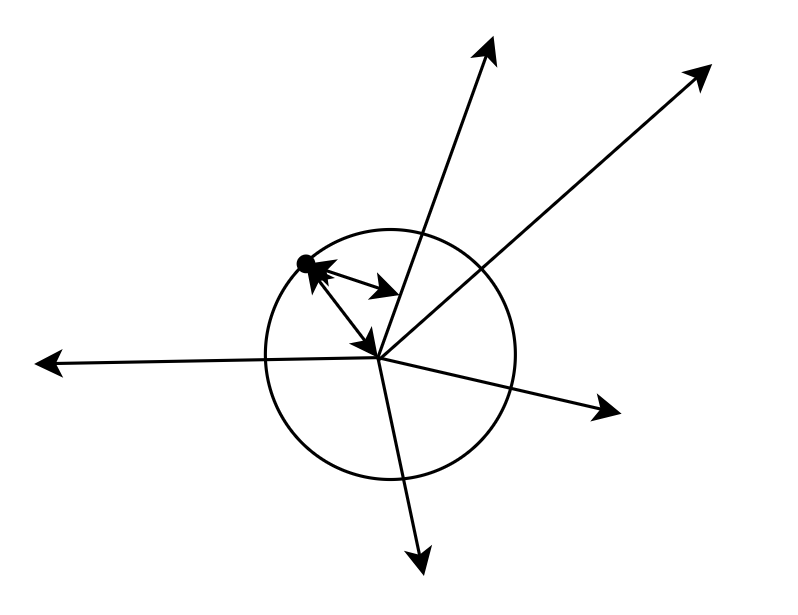
\includegraphics[scale=0.5]{figure/6.png}
    \end{figure} 
    \end{note}

\begin{theorem}
    无穷维赋范线性空间中的闭单位球不是列紧集.
\end{theorem}

\begin{proof}
    设$X$为无穷维赋范线性空间,取$x_1 \in X,\|x_1\|=1$,令$E_1 = \text{span}\{x_1\}$,则$E_1$为完备的一维子空间,由Riesz引理,存在$x_2 \in X \setminus E_1,\|x_2\|=1$,且
$$d(x_2,E_1)>\frac{1}{2}$$
令$E_2=\text{span}\{x_1,x_2\}$,则$E_2$为闭集.由Riesz引理,存在$x_3 \in X\setminus E_2,\|x_3\|=1$,且
$$d(x_3,E_2)>\frac{1}{2}$$
将此过程一直进行下去,则可得到一列$\{x_n\} \subset \overline{B}(\theta,1)$使得
$$d(x_{n+1},E_{n})>\frac{1}{2}$$
其中$E_n=\text{span}\{x_1,x_2,\cdots ,x_n\}$,于是,当$m>n$时,有$m-1 \geqslant n$且$x_n \in E_{m-1}$,所以
$$\|x_m -x_n\| \geqslant d(x_m,E_{m-1})>\frac{1}{2}$$
故$\{x_n\} \subset \overline{B}(\theta,1)$无收敛子列,从而$\overline{B}(\theta,1)$不是列紧集.
\end{proof}
\begin{note}
    该定理的主要思路是利用Riesz引理构造了一个离散的无穷点列.更为本质的是我们知道有限维赋范线性空间的闭单位球是紧的,但无穷维赋范线性空间的闭单位球不是列紧,故更不可能是紧的.
\end{note}

\begin{corollary}{\textreferencemark}
    设$X$为赋范线性空间,则:
    
    $X$是有限维赋范线性空间 $\Longleftrightarrow$ $X$\text{中闭单位球}$ \overline{B}(\theta,1)$ \text{列紧}$\Longleftrightarrow$ $X$\text{的任何有界集列紧.}
\end{corollary}

\begin{conclusion}
    有限维赋范线性空间与无穷维赋范线性空间的本质区别为:有限维赋范线性空间的任意有界集列紧,但在无穷维赋范线性空间中不成立,特别的,无穷维赋范线性空间中的单位闭球非列紧.
\end{conclusion}

\section{度量空间中的紧性}

\begin{theorem}{Hausdoff定理}
    度量空间中的列紧集一定是完全有界集.
\end{theorem}
\begin{proof}
     设$A$是度量空间$X$中的列紧集.对$\forall{\varepsilon} >0$,取$x_1 \in A$,若$A \subset B(x_1,\varepsilon)$,则$\{x_1\}$为$A$的有限$\varepsilon -$网.
     反之,$A \not\subset B(x_1,\varepsilon)$则取$x_2 \in A \setminus B(x_1,\varepsilon)$,有$d(x_1,x_2)\geqslant \varepsilon$.
     
     若$A \subset B(x_1,\varepsilon) \cup B(x_2,\varepsilon)$,则$\{x_1,x_2\}$为$A$的有限$\varepsilon -$网,否则取$x_3 \in A\setminus (B(x_1,\varepsilon) \cup B(x_2,\varepsilon))$,将此步骤重复进行下去,要么有限次终止,即$A \subset \bigcup\limits_{i=1}^{n}B(x_i,\varepsilon)$,要么不存在$A$的有限$\varepsilon -$网.

     假设$A$的无穷$\varepsilon -$网为$\{x_n\}$,则由选取的规则知$d(x_i,x_j)\geqslant \varepsilon \quad (i \not= j)$,故$\{x_n \}$ 无收敛子列,与$A$为列紧集矛盾,故$A$一定有有限$\varepsilon -$网,即$A$是完全有界集.
\end{proof}


\begin{theorem}{Hausdoff逆定理}
    在完备度量空间中的完全有界集是列紧集
\end{theorem}
\begin{proof}
    设$X$是完备度量空间,$A \subset X$是完全有界集,$\{x_n\}$是$A$中的点列,由于$A$全有界,取$\varepsilon_k=\frac{1}{k}$,$A$有有限$\varepsilon_k -$网$\{y_1^k,y_2^k,\cdots,y_{m_k}^k\}$
    $$\{x_n\} \subset A \subset \bigcup\limits_{i=1}^{m_1}B(y_i^1,1)$$
    从而$\{B(y_i^1,1)| 1\leqslant i \leqslant m_1)$中至少有一个球含有$\{x_n\}$的无穷多项,设$B(y_{i_1},1)$含有$\{x_n\}$的一个无穷子列$\{x_{1,n}\}$,又有
    $$\{x_{1,n}\} \subset A \subset \bigcup\limits_{i=1}^{m_2}B(y_i^2,\frac{1}{2})$$
    同理存在$y_{i_2}$,有$B(y_{i_2},\frac{1}{2})$含有$\{x_{1,n}\}$的无穷子列$\{x_{2,n}\}$,将此过程一直进行下去,使得$B(y_{i_m},\frac{1}{m})$含有$\{x_{m-1,n}\}$的一个无穷子列$\{x_{m,n}\}$,从而得到一列开球$B(y_{i_1},1),B(y_{i_2},\frac{1}{2}),\cdots,B(y_{i_m},\frac{1}{m})$,取$\{x_n\}$子列$\{x_{n_k}\}$,使得
    $$x_{n_k}\in \bigcap\limits_{j=1}^{k}B(y_{i_j},\frac{1}{j}) \quad k=1,2,\cdots$$
    当$k>j$时,有
    $$x_{n_k}\in B(y_{i_j},\frac{1}{j})$$
    所以
    $$d(x_{n_k},x_{n_j}) \leqslant d(x_{n_k},y_{i_j})+d(x_{n_j},y_{i_j})<\frac{2}{j}$$
    因此$\forall \varepsilon >0$,取$N >\frac{2}{\varepsilon}$,当$k>j\geqslant N$时,$d(x_{n_k},x_{n_j})< \varepsilon$,从而$\{x_{n_k}\}$是Cauchy列,由$X$完备知$\{x_{n_k}\}$收敛.
\end{proof}
\begin{note}
    
\end{note}


\begin{theorem}{Arzela-Ascol定理}
    集合$A \subset C[a,b]$列紧的充要条件是$A$是有界的等度连续集.
\end{theorem}
\begin{proof}
    必要性:设$A \subset C[a,b]$列紧,由Hausdoff定理$A$是全有界的,又由完全有界集是有界集,从而$A$有界,且对$\forall \varepsilon >0$,$A$有有限$\varepsilon-$网,$\{f_1,f_2,\cdots,f_m\}$,对$\forall 1\leqslant i \leqslant m,f_i$在$[a,b]$上一致连续,则$\exists \delta_i$,使得当$t_1,t_2\in[a,b]$且$|t_1-t_2|<\delta_i$时,有
    $$|f_i(t_1)-f_i(t_2)|<\varepsilon .$$
    取$\delta=\min\{\delta_i | 1 \leqslant i \leqslant m\}$则对$\forall f \in A,\exists i$,使得$f \in B(f_i,\varepsilon)$,当$\forall t_1,t_2 \in [a,b]$且$|t_1-t_2|<\delta$时
    $$|f(t_2)-f(t_1)|\leqslant |f(t_2)-f_i(t_2)|+|f_i(t_2)-f_i(t_1)|+|f_i(t_1)-f(t_1)|<3\varepsilon.$$
    从而$A$等度连续.

    充分性:设$A$有界且等度连续,由于完备度量空间中的全有界集是列紧的,并且$C[a,b]$完备,由Hausdoff逆定理知,只需证$A$是全有界的.

    $\forall \varepsilon >0,\exists \delta$,对$\forall f \in A,t_1,t_2 \in [a,b]$,且$|t_1-t_2|<\delta$时
    $$|f(t_2)-f(t_1)|<\varepsilon.$$
    作$[a,b]$的分割$T$
    $$T:a=t_0 < t_1 < \cdots < t_n = b.$$
    使得$\|T\| < \delta{}$,令
    $$\widetilde{A}=\{\widetilde{f}=(f(t_1),\cdots,f(t_n))|f \in A \} \subset \mathbb{R}^n.$$
    由于$A$有界,则$\exists M >0$,使得$A \subset \overline{B}(\theta,M)$,因此对$\forall f \in A$,有
    $$\|f\|=\max\limits_{a \leqslant t \leqslant b}|f(t)| \leqslant M.$$
    则
    $$\|\widetilde{f}\|=\|(f(t_1),f(t_2),\cdots,f(t_n))\|=\left(\sum\limits_{i=1}^{n}|f(t_i)|^2 \right)^{\frac{1}{2}} \leqslant \sqrt{n}M.$$
    故$\widetilde{A}$为$\mathbb{R}^n$中有界集,从而是完全有界的.所以$\widetilde{A}$有有限的$\varepsilon -$网
    $$\{\widetilde{f_i}|f_i \in A,i=1,2,\cdots,m\}$$
    下证$\{f_1,f_2,\cdots,f_m\}$是$A$的$\varepsilon -$网.对于$\forall f \in A$,存在$1 \leqslant i \leqslant m$.使得
    $$\| \widetilde{f}-\widetilde{f_i}\|<\varepsilon$$
    对$\forall t \in [a,b]$,则存在子区间$[t_{k-1},t_k]$,有$t\in [t_{k-1},t_k]$,所以
    $$|f(t)-f_i(t)|\leqslant |f(t)-f(t_k)|+|f(t_k)-f_i(t_k)|+|f_i(t_k)-f_i(t)|< 3\varepsilon$$
    即有$\|f-f_i \| < 3\varepsilon$,从而$\{f_1,f_2,\cdots,f_m\}$是$A$的有限$3\varepsilon -$网,故$A$全有界,即$A$列紧.
\end{proof}
\begin{note}
    注意有界不一定完全有界,但在欧式空间中是等价的.对于该定理,其证明方法是非常经典的$3\varepsilon$准则,这个方法在数学分析的函数项级数一致收敛性质的证明中频繁出现,大致思路是,对于需证的绝对值不等式没有明显的条件使之成立,通过三角不等式将原绝对值分成三部分,每一部分都有明显的条件使之成立不等式.该思想是简单却重要的,主要是要发掘出条件隐含的中间变量,有需要的可以再读一读数学分析的这一部分体会其思想,只要能理解该思想,则证明一致收敛的函数列可与各种运算换序便是手到擒来.
\end{note}
\begin{note}
    在上一部分,Riesz引理告诉我们,赋范线性空间的闭单位球是紧的当且仅当线性空间是有限维的,因此,给定一个特定的无穷维赋范线性空间,刻画那些紧的闭有界子集是有趣的.Arzela-Ascoli定理给出的关于$C(X)$的子空间的紧性判别准则在$l^p$有对应的结果:
    \begin{theorem}{\textreferencemark}
        当$1 \leqslant p < \infty $时,$l^p$的闭有界子集是紧的当且仅当对$\forall \: \varepsilon >0,$存在$N$使得对任意$x=\{x_n\} \in S$,在
        $$\sum\limits_{k=N}^{\infty}|x_k|^p < \varepsilon.$$
        的意义下是等度可和的.
    \end{theorem}
\end{note}

\begin{theorem}{\textreferencemark 度量空间的紧性刻画}
   对于度量空间$X$,以下三个命题等价:
    \begin{enumerate}
        \item $X$是完备的全有界集
        \item $X$是紧集
        \item $X$是自列紧集
    \end{enumerate}
\end{theorem}
\begin{note}
    以上定理是度量空间紧性的三个等价命题
\end{note}


\section{压缩映射原理及应用}
\begin{theorem}{Banach不动点定理}
    设$X$是完备的度量空间,$T:X\to X$为压缩映射,则

    (1)$T$有唯一不动点$x^*$;

    (2)对$\forall x_0 \in X$.令$x_n =Tx_{n-1}$.则$x_n \to x^*\quad (n\to \infty).$
\end{theorem}
\begin{proof}
    对$\forall x_0 \in X$,作迭代点列$\{x_n\}$,满足
    $$x_n =Tx_{n-1} \quad\quad n=1,2,\cdots$$
    由于$T$是压缩映射,故
    $$d(x_{n+1},x_n)=d(Tx_n,Tx_{n-1})\leqslant \alpha d(x_n,x_{n-1})\leqslant \cdots \leqslant \alpha^{n} d(x_1,x_0).$$
    于是当$m >n$时,有
    \begin{align*}
        d(x_m,x_n) & \leqslant d(x_m,x_{m-1})+\cdots +d(x_{n+1},x_n) \\
        & \leqslant (\alpha^{m-1}+\cdots +\alpha^{n})d(x_1,x_0) \\
        & =\alpha^{n} \frac{1-\alpha^{m-n}}{1-\alpha}d(x_1,x_0) \\
        & \leqslant \frac{\alpha^{n}}{1-\alpha}d(x_1,x_0).
    \end{align*}
    即$\{x_n\}$是Cauchy列,由$X$完备,故$\{x_n\}$收敛,令$x_n \to x^* \quad (n \to \infty)$.由$T$的连续性,$Tx_n \to Tx^* \quad (n\to \infty)$,并且有$Tx_n =x_{n+1} \to x^* \quad (n\to \infty)$,由极限的唯一性,必有$Tx^*=x^*$,即$x^*$是$T$的不动点.
    
    下证唯一性,设$y^*$也是$T$的不动点,则有
    $$d(x^*,y^*)=d(Tx^*,Ty^*)\leqslant \alpha d(x^*,y^*)$$
    由于$\alpha <1 $,故推出$x^*=y^*$,即不动点唯一.
\end{proof}



\begin{theorem}{隐函数存在定理}
    设$f(x,y)$在带状区域
    $$ B=\{(x,y)|a\leqslant x \leqslant b , -\infty < y < +\infty \}$$
    上连续,关于$y$的偏导数存在,若有$0<m \leqslant M <+\infty$,使得在区域$B$上,有
    $$m \leqslant f'_y(x,y)\leqslant M.$$
    则对任意$(x,y)\in B$,方程$f(x,y)=0$,能确定$[a,b]$上唯一连续的隐函数$y=\varphi(x)$.
\end{theorem}
\begin{proof}
    在完备度量空间$C[a,b]$上,作映射
    \begin{align*}
        T:C[a,b] & \to C[a,b] \\
        \varphi(x) & \to \varphi(x)-\frac{1}{M}f(x,\varphi(x))
    \end{align*}
    则方程$f(x,y)=0$在$[a,b]$上的连续解等价于$T$的不动点.

    下证$T$是压缩映射,对任意$\varphi_1,\varphi_2 \in C[a,b]$,存在$0 < \theta <1$,有
    \begin{align*}
        |(T\varphi_2)(x)-(T\varphi_1)(x)| & =|\varphi_2(x)-\varphi_1(x)-\frac{1}{M}[f(x,\varphi_2(x))-f(x,\varphi_1(x))]| \\
        & =|\varphi_2(x) -\varphi_1(x)-\frac{1}{M}[f'_y(x,\varphi_1(x)+\theta(\varphi_2(x)-\varphi_1(x)))](\varphi_2(x)-\varphi_1(x))| \\
        & =|\varphi_2(x)-\varphi_1(x)|\cdot |1-\frac{1}{M}[f'_y(x,\varphi_1(x)+\theta(\varphi_2(x)-\varphi_1(x)))]| \\
        & \leqslant (1-\frac{m}{M})|\varphi_2(x)-\varphi_1(x)|.
    \end{align*}
    故有
    $$d(T\varphi_2,T\varphi_1) \leqslant (1-\frac{m}{M})d(\varphi_2,\varphi_1)$$
    即$T$是压缩映射,从而$T$存在唯一不动点$\varphi \in C[a,b]$,使得$(T\varphi)(x)=\varphi(x)$

    即方程$f(x,y)=0$能确定$[a,b]$上唯一连续的隐函数$y=\varphi(x)$.
\end{proof}
\begin{theorem}{常微分方程初值问题解的存在唯一性定理}
    设$f(x,y)$在矩形区域$S=\{(x,y)| |x-x_0| \leqslant a,|y-y_0| \leqslant b\}$上连续,若$f(x,y)$关于$y$满足Lipschitz条件,即存在常数$L >0$,使得对任意的$(x,y_1),(x,y_2) \in S$,有
    $$|f(x,y_2)-f(x,y_1)| \leqslant L|y_2 -y_1|.$$
    则常微分方程初值问题
    \[	
    \begin{cases}
        \frac{dy}{dx} &= f(x,y(x)) \\
        y(x_0) & =y_0
    \end{cases}
    \]
    在区间$I=\{x||x-x_0| \leqslant h \}$上存在唯一解,其中$0 < h < \min \{a,\frac{b}{M},\frac{1}{L}\},M=\max\limits_{(x,y)\in S}|f(x,y)|.$
\end{theorem}
\begin{proof}
    将微分方程换为积分方程,则微分方程的解等价于
    $$y(x)=y_0 +\int_{x_0}^{x}f(s,y(s))ds.$$
    令$D=\{y \in C(I):\|y-y_0\| \leqslant b\},$则$D$为$C(I)$中的有界闭集,由于$C(I)$完备,故$D$完备,作$D$上的算子
    $$(Ty)(x)=y_0 + \int_{x_0}^{x}f(s,y(s))ds.$$
    则方程的解等价于$T$的不动点,因为
    $$|(Ty)(x)-y_0|=\left|\int_{x_0}^{x}f(s,y(s))ds\right| \leqslant M|x-x_0| \leqslant Mh < b$$
    所以$Ty \in D$,于是$T$是$D$到$D$自身的映射.

    下证$T$是压缩映射,对$\forall y_1,y_2 \in D$.
    \begin{align*}
        |(Ty_1)(x)-(Ty_2)(x)| & = \left|\int_{x_0}^{x}f(s,y_1(s))-f(s,y_2(s))ds\right| \\
        & \leqslant L\int_{x_0}^{x}|y_1(s) -y_2(s)|ds \\
        & \leqslant L\|y_1-y_2\| |x-x_0|  \\
        & \leqslant Lh \|y_1 -y_2 \|.
    \end{align*}
    所以$\|Ty_1 -Ty_2\| \leqslant Lh \|y_1 -y_2\|$,即$T$为$D$上的压缩映射,于是$T$存在唯一不动点$y^* \in D,Ty^* = y^*$,即
    $$y^*(x)=y_0 +\int_{x_0}^{x}f(s,y^*(s))ds$$
    故$y^*(x_0)=y_0$且$y^*(x)$在$I$上可微,求导可得
    $$\frac{dy^*(x)}{dx}=f(x,y^*(x)).$$
    因此,常微分方程初值问题在区间$I$上存在唯一解.
    
\end{proof}
\begin{note}
    利用幂压缩可将定理中的$0 < h < \min \{a,\frac{b}{M},\frac{1}{L}\}$加强到$0 < h < \min\{a,\frac{b}{M}\}$.下证$T$是幂压缩映射,
    \begin{proof}
        对$\forall y_1,y_2 \in D$.
    \begin{align*}
        |(Ty_1)(x)-(Ty_2)(x)| & = \left|\int_{x_0}^{x}f(s,y_1(s))-f(s,y_2(s))ds \right| \\
        & \leqslant L\int_{x_0}^{x}|y_1(s) -y_2(s)|ds \\
        & \leqslant L\|y_1-y_2\| |x-x_0|  \\
        & \leqslant Lh \|y_1 -y_2 \|.
    \end{align*}
    \begin{align*}
        |(T^2y_1)(x)-(T^2y_2)(x)| & = \left|\int_{x_0}^{x}f(s,Ty_1(s))-f(s,Ty_2(s))ds \right| \\
        & \leqslant L\int_{x_0}^{x}|Ty_1(s) -Ty_2(s)|ds \\
        & \leqslant L^2 \int_{x_0}^{x}\int_{x_0}^{x}|y_1(t)-y_2(t)|dt ds \\
        & \leqslant \frac{L^2 h^2}{2!} \|y_1 -y_2\|.
    \end{align*}
    由数学归纳法可得
    $$|(T^n y_1)(x)-(T^n y_2)(x)|\leqslant \frac{L^n h^n}{n!}\|y_1-y_2\|.$$
    取$n$使得$\frac{L^n  h^n}{n!} < 1$
    从而$T^n$是压缩映射,有唯一不动点,方程有唯一解.
    \end{proof}
    
\end{note}





\chapter{有界线性算子与连续线性泛函}
\section{有界线性算子}
\begin{theorem}
    设$X,Y$是赋范线性空间.\quad
     $T: X \to Y $为有界线性算子的充分必要条件是$T$是连续线性算子.
\end{theorem}
\begin{proof}
    必要性:设$T$是有界线性算子,则$\exists M>0$,使得
    $$\|Tx\|\leqslant M\|x\| \quad\quad\quad\forall x \in X.$$
    当$x_n\to \theta_X \quad (n \to \infty)$,由上式有
    $$\|Tx_n\| \leqslant M \|x_n\|\to 0 \quad\quad (n\to \infty).$$
    即$Tx_n \to \theta_Y \quad \quad (n\to \infty)$,故$T$在$x=\theta_X$连续,从而$T$在$X$上连续.

    充分性:设$T$是连续线性算子,则$T$在$x=\theta_X$处连续,取$\varepsilon_0 =1$,则$\exists \delta$,使得当$x \in B(\theta_X,\delta)\cap X$,有
    $$T(B(\theta_X,\delta)\cap X)\subset B(T\theta_X,1)\cap Y$$
    对$\forall x \in X$,当$x \not= \theta_X$时,有$\frac{\delta x}{2\|x\|} \in B(\theta_X,\delta)$,所以$T(\frac{\delta x}{2\|x\|})=Tx\cdot \frac{\delta}{2\|x\|} \in B(\theta_Y,1)\cap Y$,从而$\|Tx\|\leqslant \frac{2}{\delta}\|x\|$.
    当$x=\theta_X$时,显然成立,从而$T$有界
    
\end{proof}
\begin{note}
    此证明中用到一个引理,线性映射$T$在一点连续则全局连续,即
    \begin{lemma}
        设$X,Y$是线性空间.$T:X\to Y$是线性映射.若$T$在点$x_0$连续,则$T$在$T$上连续.
    \end{lemma}
    \begin{proof}
        $T$在$x_0$处连续,则对$\forall \varepsilon >0,\exists \delta$,当$x \in B(x_0,\delta)$时,有
        $$Tx \in B(Tx_0,\varepsilon)$$
        对任意$x \in X$有$x=x-x_0+x_0$,并且$Tx=T(x-x_0)+Tx_0.$从而当$x \in B(x,\delta)$时,即$x \in x-x_0 +B(x_0,\delta)$时,有
        $$Tx \in T(x-x_0)+TB(x_0,\delta) \subset T(x-x_0)+B(Tx_0,\varepsilon) = B(Tx,\varepsilon).$$
        从而$T$在$x$处连续,由$x$的任意性,$T$在$X$上连续.
    \end{proof}
    现在从代数结构考虑该引理的本质.对于任意线性空间$X$,$X$有两类自然的自同构,分别是伸缩变换和平移变换.考虑该引理中蕴含的平移变换,对任意$y \in X$,定义$X$上的平移变换$K_y$.
    \begin{align*}
        K_y:X & \to X \\
            x & \to x+y
    \end{align*}
    显然$K_y$是$X$的自同构映射,由于映射满足Lipschitz条件$\|K_y x_1 -K_y x_2\|=\|x_1 -x_2\|$,从而$K_y$在$X$上一致连续,故连续.则该定理的本质可以理解如下:
    $$T\text{在}x_0\text{处连续}\Longleftrightarrow(TK_y)\text{在}x_0\text{处连续} \Longleftrightarrow T\text{在}K_y x_0=x_0 + y\text{处连续} $$
    则对任意$x \in X$,取$y=x-x_0$,即可得到$T$在$x$处连续.
\end{note}

\begin{problem}
    算子范数的计算
\end{problem}
\begin{note}
    对于该类问题,我们考虑有界线性算子$T:X\to Y$,则此时需要分两步走.第一,我们需要求得算子范数的一个平凡上界$M$,此过程是平凡的,即通过算子的定义进行放缩,注意此时放缩不能过大,每次放缩时,等号要么可以成立,要么在某个极限过程下可以成立,则此时这个上界即为算子的范数.另一方面,由算子范数的等价定义,我们需要找到$\|x\|=1$或者$\|x\|\leqslant 1$使得$\|Tx\|=M$,或者找到点列$\{x_n\}$满足$\|x_n\|=1$或者$\|x_n\|\leqslant 1$使得$\lim\limits_{n\to \infty}\|Tx_n\|=M$,由算子范数的定义即得$\|T\|=M$.
\end{note}

\begin{example}
    设$K \in C([a,b]\times [a,b])$,验证从$C[a,b]$到$C[a,b]$的积分算子
    $$(S\varphi)(x)=\int_{a}^{b}K(x,y)\varphi(y)dy \quad\quad \varphi \in C[a,b]$$
    为有界线性算子,并求其范数$\|S\|$.
\end{example}
\begin{proof}
    对任意$\varphi \in C[a,b]$,有
    \begin{align*}
        |(S\varphi)(x)| &\leqslant \int_{a}^{b}|K(x,y)||\varphi(y)|dy \\
        & \leqslant \int_{a}^{b}|K(x,y)|dy \cdot \|\varphi\|
    \end{align*}
    所以
    $$\|S\varphi\|_C \leqslant \left(\max\limits_{a\leqslant x \leqslant b}\int_{a}^{b}|K(x,y)|dy \right)\cdot \|\varphi\|_{C}$$
    因此$S:C[a,b] \to C[a,b]$有界,取
    $$M=\max\limits_{a \leqslant x \leqslant b}\int_{a}^{b}|K(x,y)|dy$$
    则$\|S\| \leqslant M$,下证$\|S\|=M$.由连续函数的最值定理,存在$x_0 \in [a,b]$,使得
    $$M=\int_{a}^{b}|K(x_0,y)|dy$$
    作$[a,b]$上的函数$\varphi(y)=\text{sgn}(K(x_0,y))$,则$\varphi(y)$为$[a,b]$上的简单函数,由Lusin定理,存在$\{\varphi_n\} \subset C[a,b]$且$|\varphi_n(y)|\leqslant 1$,使得$\varphi_n(y)$在$[a,b]$上几乎处处收敛于$\varphi(y)$,从而
    $$\|S\| \geqslant \|S \varphi_n\| \geqslant (S\varphi_n)(x_0)=\int_{a}^{b}K(x_0,y)\varphi_n(y)dy$$
    当$n \to \infty$时,由控制收敛定理.
    $$\int_{a}^{b}K(x_0,y)\varphi_n(y)dy\to \int_{a}^{b}K(x_0,y)\varphi(y)dy=\int_{a}^{b}|K(x_0,y)|dy=M$$
    所以$\|S\| \geqslant M$,因此可得$\|S\|=M$,即
    $$\|S\|=\max\limits_{a\leqslant x \leqslant b}\int_{a}^{b}|K(x,y)|dy$$.

    
\end{proof}

\begin{theorem}
    设$X$为赋范线性空间,$Y$为Banach空间,则有界线性算子空间$\mathscr{B}(X,Y)$是Banach空间
\end{theorem}
\begin{proof}
    设 $\{T_n\}\subset\mathscr{B}(X,Y)$ 为 Cauchy 列.由 Cauchy 列的定义,对任意$\varepsilon>0$,存在$N=N(\varepsilon)>0$,当$m>n\geqslant N$时,有
$$\|T_m-T_n\|<\varepsilon.$$

因此,任取$x\in X$,当$m>n\geqslant N$时,有
$$
    \|T_mx-T_nx\|=\|(T_m-T_n)x\|\leqslant\|T_m-T_n\|\cdot\|x\|<\varepsilon\cdot\|x\|.\eqno (1)
$$

所以$\{T_nx\}$为$Y$中的 Cauchy 列,则其必收敛.设

$$\lim\limits_{n\to\infty}T_nx=Tx.\label{}$$



则由极限的线性性可知 $T:X\to Y$ 为线性算子.
在(1)式中让$m\to\infty$,则当$n\geqslant N$ 时,有
$$
    \|(T_n-T)x\|\leqslant \varepsilon\cdot\|x\|.\eqno(2)
$$
所以$T_n-T\in\mathscr{B}(X,Y).$从而$T=T_n-(T_n-T)\in\mathscr{B}(X,Y)$,
且由 (2) 式知当$n\geqslant N$时,$\|T_n-T\|\leqslant \varepsilon.$
因此在$\mathscr{B}(X,Y)$中$T_n\to T(n\to\infty)$, 由$\{T_n \}$ 的任意性,$\mathscr{B}(X,Y)$ 中任意 Cauchy 列收敛. 故 $\mathscr{B}(X,Y)$ 完备,为 Banach 空间.
\end{proof}

\section{Hahn-Banach}

\begin{theorem}{\textreferencemark Hahn-Banach 延拓定理,1927}
 设$X$为赋范线性空间,$G$为$X$的线性子空间,$f$为$G$上的连续线性泛函.则存在$X$上的连续线性泛函$F$,使得

$(\mathbf{i})$当$x\in G$时$,F(x)=f(x);$

$(\mathbf{ii})\|F\|=\|f\|_G.$

\end{theorem}
\begin{note}
    本课程只要求证明$X$ 比$G$ 高一维的情形,在本节末尾给出更为平凡Hahn-Banach 延拓定理的完整证明.
\end{note}

\begin{lemma}
设$X$为赋范线性空间,$A$为$X$的线性子空间,$f$为定义在$A$上的实连续线性泛函.
对任意的 $x_0\in X\setminus A$,令
$$A_1=\text{span}\{A,x_0\}=\{tx_0+x\mid x\in A,t\in\mathbb{R}\}$$

则$f$可保范地延拓为$A_1$上的实连续线性泛函$g$,即

 $(\mathbf{i})$当$x\in A$时$,g(x)=f(x)$ \\
 $(\mathbf{ii})\|g\|_{A_1}=\|f\|_A$
\end{lemma}

\begin{proof}
    $A_1$中的元素$ y $可唯一地表示为$y=x+tx_0$,其中,$x\in A$, $t\in \mathbb{R} .$

若 $y$又可表示为$y=x^\prime+t^{\prime}x_0$,其中$x^\prime\in A,t^{\prime}\in\mathbb{R}.$
如果$t\neq t^{\prime}$,则由$x+tx_0=x^{\prime}+t^{\prime}x_0$,
得$x_0=\frac1{t-t^{\prime}}(x^{\prime}-x)\in A.$
这与$x_0 \notin A$矛盾. 故$t=t^{\prime},x=x^{\prime}$,即表示唯一.

现在我们分析$f$在$A_1$上延拓的形成.

 若线性泛函$g$是$f$在$A_1$上的延 拓,则当$x\in A$时,应当满足:
$$g(x+tx_0)=f(x)+tg(x_0).$$

取$c\in\mathbb{R}$,定义$A_1$上的泛函 g:
$$
    g(x+tx_0)=f(x)+tc,\quad x\in A,\:t\in\mathbb{R}.\eqno(1)
$$
    由$A_1$中的元素 $x+tx_0$ 分解的唯一性可知 $g$ 在$A_1$上有定义.易验证这样定义的$g$ 为$A_1$上的线性泛函且$(\mathbf{i})$成立.现在我们选适当的$c$,使得
$$
    |f(x)+tc|\leqslant\|f\|_A\cdot\|x+tx_0\|,\quad x\in A,\:t\in\mathbb{R}.\eqno (2)
$$

这只需证明
$$
    f(x)+tc\leqslant\|f\|_A\cdot\|x+tx_0\|,\quad x\in A,\:t\in\mathbb{R}.\eqno(3)
$$

在上式中用$-x,-t$代替$x,t$得
$$
    f(x)+tc\geqslant-\|f\|_A\cdot\|x+tx_0\|.\eqno(4)
$$

由(3)式和(4)式可得(2)式.

下面讨论如何通过选取恰当的 $c$,使得(3)式成立.

显然,当$t=0$时,(3) 式对任意的$c$均成立

当$t>0$时,令$u=\frac{1}{t}x$,由(3)式得
$$
    c\leqslant\|f\|_A\cdot\|u+x_0\|-f(u),\quad u\in A.\eqno(5)
$$

当$t<0$ 时,令 $u^\prime=-\frac{1}{t}x$,由(3)式得
$$
    c\geqslant f(u')-\|f\|_A\cdot\|u'-x_0\|,\quad u'\in A.\eqno(6)
$$

同理,当$t<0$时,令$u=\frac{1}{t}x$,由(4)式得
$$
    c\leqslant\|f\|_A\cdot\|u+x_0\|-f(u),\quad u\in A.\eqno(5^\prime)
$$

当$t>0$ 时,令 $u^\prime=-\frac{1}{t}x$,由(4)式得
$$
    c\geqslant f(u')-\|f\|_A\cdot\|u'-x_0\|,\quad u'\in A.\eqno(6^\prime)
$$


因此只要选$c$,使得$ (5)(5^\prime)(6)(6^\prime)$式同时成立,则(2)式成立.

下面证明可以取到使$(5)(5^\prime)(6)(6^\prime)$式同时成立的$c.$

对任意$u,u^\prime\in A$,有
$$\begin{aligned}f(u)+f(u^{\prime})&=f(u+u^{\prime})\leqslant|f(u+u^{\prime})|\\&\leqslant\|f\|_A\cdot\|u+u^{\prime}\|\\&\leqslant\|f\|_A(\|u+x_0\|+\|u^{\prime}-x_0\|).\end{aligned}$$

所以
$$
    f(u')-\|f\|_A\cdot\|u'-x_0\|\leqslant\|f\|_A\cdot\|u+x_0\|-f(u).\eqno(7)
$$

令
$$m(x_0)=\sup_{u'\in A}\{f(u')-\|f\|_A\cdot\|u'-x_0\|\},$$
$$M(x_0)=\inf_{u\in A}\{\|f\|_A\cdot\|u+x_0\|-f(u)\}.$$

则由 (7)式得$m(x_0)\leqslant M(x_0)$.故可取$c$,使得$$m(x_0)\leqslant c\leqslant M(x_0).$$

对这样的$c$,$(5)(5^\prime)(6)(6^\prime)$式均成立,从而(2)式成立.故$g$为$A$上的连续线性泛函,且 $\|g\|_{A_1}\leqslant\|f\|_A.$

又因为线性泛函延拓时范数不会减少,即$\|g\|_{A_1}\geqslant\|f\|_A.$综合得$\|g\|_{A_1}=\|f\|_A.$
\end{proof}



\begin{note}
     当$m(x_0)=M(x_0)$时,$c$仅可取一个值,此时保范延拓唯一;当$m(x_{0})<M(x_{0})$ 时$,c$ 可取无穷多个值,此时保范延拓 $g$ 有无穷多个.因此一般来说,$f$ 的延拓不唯一.
\end{note}

\begin{theorem}{泛函存在定理}
    设$X$是赋范线性空间,$G$为$X$上的线性子空间.若
$$d_0=d(x_0,G)>0,\quad x_0\in X \setminus G .$$
则存在$X$上的连续线性泛函$f$,满足

(1)当$x\in G$时$,f(x)=0$;

(2)$f(x_0)=d(x_0,G)$;

(3)$\left\|f\right\|=1.$
\end{theorem}
\begin{proof}
    令$G_1=$span$\{G,x_0\}.$ 则$G_1$ 中元素可唯一地表示成
$$y=x+tx_0,\quad x\in G,t\in\mathbb{R}.$$
定义$G_1$上的泛函 $f_1(x+tx_0)=td_0.$则$f_{1}$为$G_1$上的线性泛函,且满足条件 (1)和 (2).当$t\neq 0$时,有
$$\|x+tx_0\|=|t|\cdot\left\|x_0-\left(-\frac1tx\right)\right\|\geqslant|t|\cdot d_0.$$
因此有
$$|f_1(x+tx_0)|=|t|\cdot d_0\leqslant\|x+tx_0\|.$$
所以$\|f_1\|_{G_1}\leqslant 1.$
另一方面,由$d_0=d(x_0,G)$的定义,存在$\{x_n\}\subset G$,使得
$$\|x_0-x_n\|\to d_0,\quad n\to\infty.$$
从而
\begin{align*}
    d_0=|f_1(x_0)|& =|f_1(x_0)-f_1(x_n)| \\
    & =|f_1(x_0-x_n)| \\
    & \leqslant\|f_1\|_{G_1}\cdot\|x_0-x_n\|.
\end{align*}
令$n \to \infty $可得$\|f_1\|_{G_1} \geqslant 1.$故$f_1$满足条件 (3).由Hahn-Banach延拓定理知
$f_{1}$可保范地延拓为$X$上的连续线性泛函 $f$,
且$f$满足条件(1)(2)及(3).
\end{proof}
\begin{note}
    
\end{note}


\begin{theorem}{泛函存在定理}
    设$X$是赋范线性空间,$x_0\in X,x_0\neq\theta.$ 则存在 $f\in X^*$,满足

$(1)f(x_0)=\|x_0\|;$

$(2)\left\|f\right\|=1.$
\end{theorem}
\begin{proof}
    令$G=\text{span}\{x_0\}$,则$G$中元素可被唯一表示为
    $$y=tx_0 ,\quad t \in \mathbb{R}.$$
    定义$G$上的泛函$f_1(tx_0)=t\|x_0\|$,则$f_1$是线性泛函并且满足条件(1),当$t\not= 0$时
    $$|f_1(tx_0)|=|t|\cdot \|x_0\|=\|tx_0\|.$$
    从而有$\|f_1\|_{G}=1$,故$f_1 \in X^*$并且满足条件(2),由Hahn-Banach延拓定理$f_1$可延拓为$X$上的连续线性泛函$f$并且满足条件(1)(2).
\end{proof}
\begin{note}
    或上一定理中取$G=\{\theta\}$即可得证
\end{note}

\begin{theorem}{\textreferencemark Hahn-Banach 定理}
设泛函$p:E\to\mathbb{R}$满足
$$\begin{aligned}&p(\lambda x)=\lambda p(x),\quad\forall x\in E,\forall\lambda>0,\\&p(x+y)\leqslant p(x)+p(y),\quad\forall x,y\in E,\end{aligned}$$
设$G\subset E$为线性子空间,$g:G\to\mathbb{R}$为线性泛函使得
$$g(x)\leqslant p(x),\quad\forall x\in G.$$
那么,存在一个定义在$E$上的线性泛函$f$,它为$g$在$E$上的扩张,即,$g(x)=f(x),\forall x\in G$,且
$$f(x)\leqslant p(x),\quad\forall x\in E.$$

\end{theorem}
\begin{proof}
令
$$P=\left\{(H,\ell)\left|\begin{array}{l}H\text{ 为 }E\text{ 的子空间且 }G\subset H\\\ell\text{ 为 }H\text{ 上的线性泛函}\\\ell|_G=g,\ell(x)\leqslant p(x),\forall x\in H\end{array}\right.\right\}$$
在 $P$ 上定义关系$\leqslant$如下
$$(H_1,\ell_1)\leqslant(H_2,\ell_2)\Leftrightarrow H_1\subset H_2,\:\ell_2|_{H_1}=\ell_1.$$
则 $(P,\leqslant)$ 为偏序集.

\textbf{断言}:$(P,\leqslant)$ 是归纳的.

由\textbf{断言},根据 Zorn 引理,存在$(P,\leqslant)$的一个极大元$(H_0,\ell_0).$下证:$H_0=E.$
 
否则,存在$x_0\in E$,但$x_0\notin H_0.$考虑$E$的子空间$H_1=H_0+\mathbb{R}x_0.$我们希望选取某个适
当的$\alpha\in\mathbb{R}$使得线性泛函
$$\ell_1:H_0+\mathbb{R}x_0\to\mathbb{R},\:h_0+tx_0\mapsto\ell_0(h_0)+t\alpha,$$
满足
$$\ell_1(h_0+tx_0)\leqslant  p(h_0+tx_0),\:\forall h_0\in H_0,\forall t\in\mathbb{R}. \eqno (1)$$
明显的,$\ell_1$ 是线性泛函.事实上,对任何的 $h_0^1,h_0^2\in H_0,t_1,t_2\in\mathbb{R}$,有
$$\begin{aligned}\ell_{1}\left((h_{0}^{1}+t_{1}x_{0})+(h_{0}^{2}+t_{2}x_{0})\right)=&\ell_1(h_0^1+h_0^2+(t_1+t_2)x_0)=\ell_0(h_0^1+h_0^2)+(t_1+t_2)\alpha\\=&\ell_0(h_0^1)+\ell_0(h_0^2)+t_1\alpha+t_2\alpha=\ell_0(h_0^1)+t_1\alpha+\ell_0(h_0^2)+t_2\alpha\\=&\ell_1(h_0^1+t_1\alpha_0)+\ell_1(h_0^2+t_2x_0).\end{aligned}$$
下面,我们将证明存在适当的$\alpha\in\mathbb{R}$,使得 (1)成立,即
$$\ell_0(h_0)+t\alpha=\ell_1(h_0+tx_0)\leqslant  p(h_0+tx_0),\:\forall h_0\in H_0,\forall t\in\mathbb{R}.\eqno (2)$$

(i) 若$t=0$,对任何的$\alpha$均适用(2).

(ii) 若$t>0,(2)$两端同时除以$t$,得到
$$\ell_0\left(\dfrac{1}{t}h_0\right)+\alpha\leqslant  p\left(\dfrac{1}{t}h_0+x_0\right),\:\forall h_0\in H_0.$$
这等价于
$$\ell_0(h_0)+\alpha\leqslant  p(h_0+x_0),\:\forall h_0\in H_0.$$
即
$$\alpha\leqslant  p(h_0+x_0)-\ell_0(h_0),\:\forall h_0\in H_0.$$

(iii) 若$t<0,(2)$两端同时除以$-t$,得到
$$\ell_0\left(-\dfrac{1}{t}h_0'\right)-\alpha\leqslant \dfrac{1}{-t}p(h_0'+tx_0)=p\left(-\dfrac{1}{t}h_0'-x_0\right).$$
这等价于
$$\ell_0(h_0')-\alpha\leqslant  p(h_0'-x_0).$$
即
$$-\alpha\leqslant  p(h_0'-x_0)-\ell_0(h_0'),\:\forall h_0'\in H_0.$$
也即
$$\ell_0(h_0')-p(h_0'-x_0)\leqslant \alpha,\:\forall h_0'\in H_0.$$
综上 (i), (ii), (iii), 我们需要得到
$$\ell_0(h_0')-p(h_0'-x_0)\leqslant \alpha\leqslant  p(h_0+x_0)-\ell_0(h_0),\:\forall h_0,h_0'\in H_0.\eqno (3)$$
此即要证
$$\ell_0(h_0')+\ell_0(h_0)\leqslant  p(h_0'-x_0)+p(h_0+x_0).$$
而
$$\ell_0(h_0')+\ell(h_0)=\ell_0(h_0'+h_0)\leqslant  p(h_0'+h_0)\leqslant  p(h_0'-x_0)+p(h_0+x_0).$$
因此 (3) 中的 $\alpha$ 始终存在.

由上分析,我们得到存在$\alpha\in\mathbb{R}$使得
$$\sup\limits_{h_0'\in H_0}\left[\ell_0(h_0')-p(h_0'-x_0)\right]\leqslant \alpha\leqslant \inf\limits_{h_0\in H_0}\left[p(h_0+x_0)-\ell_0(h_0)\right],$$
以及
$$\ell:H_0+\mathbb{R}x_0\to\mathbb{R},\:h_0+tx_0\mapsto\ell_0(h_0)+t\alpha $$
成为一个线性泛函且$\ell_1(h_0+tx_0)\leqslant  p(h_0+tx_0),\forall h_0\in H_0,\forall t\in\mathbb{R}.$由$\ell_1$的定义知$\ell_1|_{H_0}=\ell_0.$
即 $(H_1,\ell_1)\in P$,且 $(H_0,\ell_0)\lneqq (H_1,\ell_1)$.这与 $(H_0,\ell_0)$ 为极大元相矛盾!定理得证.
\end{proof}
\begin{note}
    断言的证明:明显的,$(P,\leqslant )$ 是偏序集.设$Q\subset P$为$P$的一个全序子集.记$Q=\{(H_{\alpha},\ell_{\alpha})\mid\alpha\in\Gamma\}$,其中$\Gamma$为指标集.定义
$$H=\bigcup\limits_{\alpha\in\Gamma}H_\alpha,\quad\ell(x)=\ell_\alpha(x),\:\text{若}\:x\in H_\alpha.$$
我们将证明 $(H,\ell)\in P$ 且它为$Q$ 的一个上界.

事实上,$(1)\quad G\subset H$是显然的. 另外,对任何的$x,y\in H$,必定存在$\alpha,\beta\in\Gamma$使得$x\in H_{\alpha}\in Q,y\in H_{\beta}\in Q$,而$Q$是全序集,那么要么有$H_\alpha\subset H_{\beta}$,要么$H_{\beta}\subset H_{\alpha}$,不妨设为$H_{\alpha}\subset H_{\beta}$,从而$x,y\in H_{\beta}$,于是$ax+by\in H_{\beta}\left(\forall a,b\in\mathbb{R}\right).$于是$ax+by\in H.$即证得$H$是向量空间.(2) 由 $\ell(x)=\ell_\alpha(x)$ ($x\in H_\alpha)$ 以及$\leqslant $的定义知道$\ell$ 为 $H$ 上的线性泛函.(3)由 $P$ 的定义知对任何的$x\in H_\alpha$均有$\ell_\alpha(x)\leqslant  p(x)$,从而$\ell(x)\leqslant  p(x)$ $(\forall x\in H).$

综上,即证得 $(P,\leqslant )$ 是归纳的.
\end{note}


\section{共轭空间及其表示}
\begin{example}
    $\mathbb{R}^n$的共轭空间$(\mathbb{R}^n)^*$是$\mathbb{R}^n.$
\end{example}
    
\begin{proof}
     设$f\in(\mathbb{R}^n)^*,\{e_1,e_2,\cdots,e_n\}$为$\mathbb{R}^n$中的标准正交基,
其中$e_k=(0,0,\cdots,0,1,0,\cdots,0),k=1,2,\cdots,n.$
对任意$x=(x_1,\cdots,x_n)\in\mathbb{R}^n$且$x=\sum\limits_{k=1}^{n}x_k e_k$
有
$$f(x)=\sum_{k=1}^nx_kf(e_k).$$
令$\alpha_f=(f(e_1),f(e_2),\cdots,f(e_n))\in\mathbb{R}^n.$则
$$f(x)=x\cdot\alpha_f. \eqno (1)$$
且有
$$|f(x)|\leqslant\|\alpha_f\|\cdot\|x\|.$$
所以$\|f\|\leqslant\|\alpha_f\|.$又因为
$$f(\alpha_f)=\alpha_f\cdot\alpha_f=\|\alpha_f\|^2.$$
因此
$$\|f\|\geqslant\frac{|f(\alpha_f)|}{\|\alpha_f\|}=\|\alpha_f\|\quad(\alpha_f\neq\theta).$$
所以$\|f\|=\|\alpha_f\|.$作$(\mathbb{R}^n)^*$到$\mathbb{R}^n$的映射$T$如下:
$$T:f\mapsto\alpha_f.$$
则$T$ 是线性保范映射.对任意 $x\in\mathbb{R}^n$,由(1)定义了$\mathbb{R}^n$ 上的连续线性泛函$f.$

所以,$T:(\mathbb{R}^n)^*\to\mathbb{R}^n$ 为线性保范同构.
\end{proof}

\begin{theorem}
    当$1 \leqslant p < \infty$时,有$ (l^p)^*\cong l^q$,但$l^{\infty} \ncong l^1$.
\end{theorem}
\begin{theorem}
    当$1 \leqslant p < \infty$时,有$(L^p[a,b])^*\cong L^q[a,b]$,但$(L^{\infty}[a,b])^* \ncong L[a,b]$
\end{theorem}
\begin{theorem}
    $l^1$的共轭空间$(l^1)^*$是 $l^\infty$,即对任意的 $f\in(l^1)^*$ 存在唯一的$\eta=(\eta_1,\eta_2,\cdotp\cdotp\cdotp,\eta_n,\cdotp\cdotp\cdotp)\in l^\infty$,使得$f$可以表示为
$$f( x) = \sum\limits _{n= 1}^\infty \eta _nx_n, \forall x= ( x_1, x_2, \cdots , x_n, \cdots ) \in l^1$$
且$\|f\|=\|\eta\|_\infty.$
\end{theorem}
\begin{proof}
记$e_n=(0,\cdots,0,1,0,\cdots),n=1,2,\cdots.$设$f\in(l^1)^*.$对任意$x=(x_1,\cdots,x_n,\cdots)\in l^1$,则
$$\sum_{k=1}^{n}x_{k}e_{k}\to x,\quad (n\to\infty). $$
由$f$的连续性和线性性可知
$$f(x)=\lim_{n\to\infty}f\left(\sum_{k=1}^nx_ke_k\right)=\lim_{n\to\infty}\sum_{k=1}^nx_kf(e_k)=\sum_{n=1}^\infty x_nf(e_n).\eqno (1)$$
令 $\eta_n=f(e_n),n=1,2,\cdots.$则 $|\eta_n|\leqslant\|f\|\|e_n\|_1=\|f\|.$所以$\eta=(\eta_1,\eta_2,\cdots,\eta_n,\cdots)\in l^\infty$且
$$\|\eta\|_\infty\leqslant\|f\|. \eqno (2)$$
由(1)式,$f$可表示为
$$f(x)=\sum_{n=1}^{\infty}\eta_nx_n.\eqno (3)$$
所以,对任意 $x=(x_1,\cdots,x_n,\cdots)\in l^1$,有
$$|f(x)|\leqslant\|\eta\|_\infty\sum_{n=1}^\infty|x_n|=\|\eta\|_\infty\|x\|_1. $$
因此
$$\|f\|\leqslant\|\eta\|_{\infty}.\eqno (4)$$
由(2)式及(4)式可得
$\|f\|=\|\eta\|_\infty.$
反之,对任意$\eta=(\eta_1,\eta_2,\cdots,\eta_n,\cdots)\in l^\infty$,

由(3)式定义了$l^1$上连续线性泛函.

\end{proof}

\begin{theorem}
    设 $1<p<\infty$,则 $l^p$的共轭空间$(l^p)^*$是 $l^q$,其中$\frac{1}{p}+\frac{1}{q}=1$.即对任意的 $f\in(l^p)^*$,存在唯一的 $\eta=(\eta_1,\eta_2,\cdots,\eta_k,\cdots)\in l^q$,使得 $f$可以表示为$$f(x)=\sum\limits_{k=1}^{\infty}\eta_{k}x_{k},\forall x=(x_{1},x_{2},\cdots,x_{k},\cdots)\in l^{p}\eqno(1)$$
    且$\|f\|=\|\eta\|_{q}$.
\end{theorem}
\begin{proof}
    设$f\in(l^{p})^{*}$令$\eta_{k}=f(e_{k}),k=1,2,\cdots$.先证 $\eta=(\eta_{1},\eta_{2},\cdots\eta_{k},\cdots)\in l^{q}$. 考察
    \begin{align*}
        x^{(n)} & =(|\eta_{1}|^{q-1}\cdot\mathrm{sgn}\eta_{1},|\eta_{2}|^{q-1}\cdot\mathrm{sgn}\eta_{2},\cdots,|\eta_{n}|^{q-1}\cdot\mathrm{sgn}\eta_{n},0,\cdots)\\
        &=\quad\sum\limits_{k=1}^{n}(|\eta_{k}|^{q-1}\cdot\mathrm{sgn}\eta_{k})e_{k}\in l^{p}.
    \end{align*}
    由$f$的线性性,有
$$f(x^{(n)})=f\Big(\sum\limits_{k=1}^{n}(|\eta_{k}|^{q-1}\cdot\mathrm{sgn}\eta_{k})e_{k}\Big)=\sum\limits_{k=1}^{n}|\eta_{k}|^{q}.$$
从而
$$|f(x^{(n)})|\leqslant\|f\|\cdot\|x^{(n)}\|_{p}=\|f\|\Big(\sum\limits_{k=1}^{n}|\eta_{k}|^{(q-1)p}\Big)^{\frac{1}{p}}=\|f\|\Big(\sum\limits_{k=1}^{n}|\eta_{k}|^{q}\Big)^{\frac{1}{p}}.$$
所以
$$\Big(\sum\limits_{k=1}^n|\eta_k|^q\Big)^{\frac{1}{q}}\leqslant\|f\|.$$
令$n\to \infty$,因此$,\eta\in l^q$ 且 $\|\eta\|_q\leqslant\|f\|.$此时,对任意的$x=(x_1,x_2,\cdots x_n,\cdots)\in l^p$,由 Hölder 不等式可得
$$\sum\limits_{k=1}^{\infty}|\eta_{k}x_{k}|\leqslant\Big(\sum\limits_{k=1}^{\infty}|\eta_{k}|^{q}\Big)^{\frac{1}{q}}\Big(\sum\limits_{k=1}^{\infty}|x_{k}|^{p}\Big)^{\frac{1}{p}}=\|\eta\|_{q}\|x\|_{p}.$$
因 此 ,  $\sum\limits_{k= 1}^{\infty }\eta _{k}x_{k}$ 是 绝 对 收 敛 的 . 从 而 由  $f$ 的 线 性 性 及  $x= \lim\limits _{n\to \infty }\sum\limits _{k= 1}^{n}x_{k}e_{k}$ 可 得  

$$f(x)=\lim\limits_{n\to\infty}f\Big(\sum\limits_{k=1}^{n}x_{k}e_{k}\Big)=\sum\limits_{k=1}^{\infty}\eta_{k}x_{k}.$$
因此$$|f(x)|\leqslant\sum\limits_{k=1}^{\infty}|\eta_{k}x_{k}|\leqslant\left(\sum\limits_{k=1}^{\infty}|\eta_{k}|^{q}\right)^{\frac{1}{q}}\left(\sum\limits_{k=1}^{\infty}|x_{k}|^{p}\right)^{\frac{1}{p}}=\|\eta\|_{q}\|x\|_{p}.$$
所 以  $\| f\| \leqslant \| \eta \| _q.$ 综 上 可 得  $\| f\| = \| \eta \| _q.$ 因 此 , 对 任 意  $f\in ( l^p) ^*$,存 在 唯 一 $\eta = ( \eta _1, \eta _2, \cdots \eta _k, \cdots ) \in l^q$,使得(1)式成立且$\|f\|=\|\eta\|_q.$反之,对任意$\eta\in l^q$,
(1)式确定了$l^p$上的一个连续线性泛函所以,$(l^p)^*$与$l^q$通过(1)式同构   
\end{proof}

\begin{theorem}{\textreferencemark}
    设 $1\leqslant p,q<\infty,\frac1p+\frac1q=1$,则
$$(L^p[a,b])^*=L^q[a,b].$$
即对任意的$f\in(L^p[a,b])^*$,存在唯一的$\psi\in L^q[a,b]$,使得
$$f(\varphi)=\int_a^b\varphi(t)\psi(t)dt,\quad\forall \:\varphi\in L^p[a,b] \eqno(1)$$
且$\|f\|=\|\psi\|_q.$
\end{theorem}
\begin{proof}
    要证$L^p[a,b]$上任一连续泛函都可表示成 (1)式的形式,即要找到$\psi\in L^q[a,b]$使得 (1) 成立.下面,我们分4步完成证明.

({\romannumeral1})首先证明(1) 式对特征函数所张成的函数都成立,为此取
$$A=\{\chi_{[a,t]}|\chi_{[a,t]}\text{为}[a,t]\text{上的特征函数},a\leqslant t\leqslant b\}\subset L^p[a,b].$$
将$\chi_{[a,t]}$代入(1)式,有
$$f(\chi_{[a,t]})=\int_{a}^{t}\psi(s)ds. \eqno(2)$$
令$g( t) = f( \chi _{[a,t] }).$则$g(t)$在$[a,b]$上有定义.若能证明$g(t)$绝对连续,则$\psi(t)=g^{\prime}(t)$且(2)式成立.设
$$g(t)=f(\chi_{[a,t]}),\quad t\in[a,b],\:f\in\left(L^p[a,b]\right)^*.$$

下证$g(t)$在$[a,b]$上绝对连续. 对任意$\varepsilon>0$,
设 $\{(a_i,b_i)\mid1\leqslant i\leqslant n\}$ 为$[a,b]$ 中的一组互不相交的开区间.
令$\eta_i=$sgn$(g(b_i)-g(a_i)).$则
\begin{align*}
    \sum\limits_{i=1}^{n}|g(b_{i})-g(a_{i})|=\sum\limits_{i=1}^{n}\eta_{i}(g(b_{i})-g(a_{i})) & =\sum\limits_{i=1}^{n}\eta_{i}f(\chi_{[a,b_{i}]}-\chi_{[a,a_{i}]}) \\
    &=f\Big(\sum_{i=1}^{n}\eta_{i}\chi_{[a_{i},b_{i}]}\Big) \\
    & \leqslant\|f\|\cdot\Big\|\sum_{i=1}^{n}\eta_{i}\chi_{[a_{i},b_{i}]}\Big\|_{p} \\
    & \leqslant\|f\|\cdot\Big(\int_{\bigcup\limits_{i=1}^{n}[a_{i},b_{i}]}1^{p}\Big)^{\frac{1}{p}} \\
    & =\|f\|\cdot\Big(\sum_{i=1}^{n}(b_{i}-a_{i})\Big)^{\frac{1}{p}} \\
    & <\varepsilon.
\end{align*}
所以$g(t)$在$[a,b]$上绝对连续.故$g(t)$在$[a,b]$上几乎处处可导,$g^{\prime}(t)$ 在 $[a,b]$上可积,且有Newton-Leibniz 公式
$$\int_{t_1}^{t_2}g'(s)ds=g(t_2)-g(t_1). \eqno(3)$$
令$\psi(t)=g^\prime(t)\left(g^{\prime}(t)\text{ 不存在时,取 0 值}\right)$则$\psi\in L[a,b]$,且由(3)式有
$$f(\chi_{[a,t]})=\int_{a}^{b}\chi_{[a,t]}(s)\psi(s)ds.\eqno (4)$$
记$A^{\prime}=\text{span}\{\chi_{[a,t]}| a\leqslant t\leqslant b\}.$则由(4)式及$f$的线性性,对任意$\varphi\in A^{\prime},(1)$ 式成立.


({\romannumeral2})下面证明对$[a,b]$上的有界可测函数$\varphi$,(1)式成立.设 $| \varphi ( t) | \leqslant M$, $M> 0$是常数.用$A^{\prime}$中的点列逼近$\varphi$.对任意$\frac1n$,由Lusin定理,存在$V_n\in C[ a, b]$ 及闭集$F_n\subset[a,b]$,
使得
$$m([a,b]\backslash F_n)<\frac1n.$$
 当$t\in F_n$时,有$\varphi(t)=V_n(t).$ 则$| V_n( t) | \leqslant M$, $t\in [ a, b] .$ 对 $V_n\in C[a,b]$,可用$[a,b]$ 上的阶梯函数逼近. 存在$[a,b]$的分划$$\Delta:a=t_0<t_1<\cdots<t_n=b.$$
 $V_n$关于 Δ对应的阶梯函数为
$$\varphi_n(t)=V_n(t_1)\chi_{[t_0,t_1]}+\sum\limits_{k=2}^nV_n(t_k)(\chi_{[a,t_k]}-\chi_{[a,t_{k-1}]}),$$
使得 
$$|\varphi_n(t)-V_n(t)|<\frac1n.$$ 
下证$\varphi_n$依测度一致收敛到$\varphi.$ 对$\sigma>0$,当$n$充分大使得$\frac1n<\sigma$时,有
\begin{align*}
    |\varphi_n(t)-\varphi(t)|& \leqslant|\varphi_n(t)-V_n(t)|+|V_n(t)-\varphi(t)| \\
    & <\dfrac{1}{n}+|V_n(t)-\varphi(t)| \\
    & <\sigma.\:t\in F_n.
\end{align*}
所以
$E[|\varphi_n-\varphi|\geqslant\sigma]\subset[a,b]\backslash F_n.$从而$$mE[ | \varphi _n- \varphi | \geqslant\sigma ] \leqslant m( [ a, b] / F_n) < \frac 1n\to 0 ( n\to \infty ) .$$

因此$\varphi_n$依测度一致收敛到$\varphi.$又因为$|\varphi_n(t)|\leqslant\|V_n\|_C\leqslant M.$所以$$f(\varphi_{n})=\int_{a}^{b}\varphi_{n}(t)\psi(t)dt.\eqno (5)$$
由 Lebesgue 有界收敛定理,$\varphi_n$在$L^p[a,b]$上收敛于$\varphi.$所以
$$\int_{a}^{b}\varphi_{n}(t)\psi(t)dt\to\int_{a}^{b}\varphi(t)\psi(t)dt\quad(n\to\infty).$$
在 (5) 式中,让$n\to\infty$,由$f$的连续性,有
$$f(\varphi)=\int_a^b\varphi(t)\psi(t)dt.$$

({\romannumeral3})现在证明$\psi\in L^q[a,b].$
当$p=1$时,$q=+\infty$.此时对任意$a\leqslant t_{1}\leqslant t_{2}\leqslant b$,有
$$|g(t_2)-g(t_1)|=|f(\chi_{[t_1,t_2]})|\leqslant\|f\|\cdot\|\chi_{[t_1,t_2]}\|_1=\|f\|\cdot(t_2-t_1).$$
当$g$在 $t_1$ 点可导时,$|g^\prime(t_1)|\leqslant\|f\|.$ 所以$| \psi ( t) | \leqslant \| f\| .$ 故$\psi\in L^\infty[a,b].$ 当$p>1$时,对任意的$n$,作有界可测函数
$$h_n(t)=\left\{\begin{array}{ll}|\psi(t)|^{q-1}\cdot\operatorname{sgn}\psi(t),&|\psi(t)|^q<n,\\[2ex]n|\psi(t)|^{-1}\cdot\operatorname{sgn}\psi(t),&|\psi(t)|^q\geqslant n.\end{array}\right.$$
则$h_n(t)$为有界可测函数,由情形{{\romannumeral2}}有
$$f(h_n)=\int_a^bh_n(t)\psi(t)dt=\int_a^b[|\psi(t)|^q]_ndt.$$
从而$$|f(h_n)|\leqslant\|f\|\cdot\|h_n\|_p\leqslant\|f\|\cdot\left(\int_a^b[|\psi(t)|^q]_ndt\right)^{\frac1p}.$$ 
所以
$$\int_a^b[|\psi(t)|^q]_ndt\leqslant\|f\|^q$$
且
$$\int_a^b|\psi(t)|^qdt\leqslant\|f\|^q.$$ 
所以$\psi\in L^q[a,b]$且令$n\to\infty$可得

$$\|\psi\|_q\leqslant\|f\|.\eqno (6)$$

({\romannumeral4})最后证明对任意$\varphi\in L^p[a,b],(1)$式成立.由$B_p[a,b]$在$L^p[a,b]$中的稠密性,存在$[a,b]$上一列有界可测函数$\{\varphi_n(t)\}$,使得$\varphi_n\xrightarrow{\|\cdot\|_p}\varphi(n\to\infty).$

在 $f( \varphi _n) = \int _a^b\varphi _n( t) \psi ( t) dt$ 中令$n\to\infty$,结合 $f$的连续性可得 $$f(\varphi)=\int_a^b\varphi(t)\psi(t)dt.$$
因此,当$n\to\infty$时,有
$$\left|\int_{a}^{b}\varphi_{n}(t)\psi(t)dt-\int_{a}^{b}\varphi(t)\psi(t)dt\right|\leqslant\int_{a}^{b}|\varphi_{n}-\varphi|\cdot|\psi|dt\leqslant\|\varphi_{n}-\varphi\|_{p}\cdot\|\psi\|_{q}\to 0.$$
故(1) 式成立,且由 Hölder 不等式,有
$$|f(\varphi)|=\Big|\int_{a}^{b}\varphi(t)\psi(t)dt\Big|\leqslant\|\varphi\|_{p}\cdot\|\psi\|_{q}.$$
所以$\|f\|\leqslant\|\psi\|_q$,结合(6)式可得,$\|f\|=\|\psi\|_q.$
综合上述 ({\romannumeral1}),({\romannumeral2}),({\romannumeral3}),({\romannumeral4}),证得此定理成立.
\end{proof}
\begin{note}
    当$p=\infty$时,上述定理的结论不成立. 即
 $(L^\infty[a,b])$的共轭空间不是$L^1[a,b].$
\end{note}
\begin{note}
    对可测的$E\subset\mathbb{R}^n$,有与上述定理对应的结论.
\end{note}
\begin{corollary}{\textreferencemark}
设 $1\leqslant p,q<\infty,\frac1p+\frac1q=1$,则
$$(L^p(E))^*=L^q(E)$$
即对任意的$f\in(L^p(E))^*$,存在唯一的$\psi\in L^q(E)$,使得
$$f( \boldsymbol{\varphi }) = \int _E\boldsymbol{\varphi }( x) \boldsymbol{\psi }( x) dt \quad\quad \forall\varphi\in L^p(E)$$
且$\|f\|=\|\psi\|_q.$
\end{corollary}


\begin{theorem}{\textreferencemark}
     $C[a,b]$的共轭空间$C[a,b]^*=\bigvee\limits_0[a,b]$, 即对任意的$f\in C[a,b]^*$,则存在唯一的$g\in \bigvee\limits_0[a,b]$,使得
$$f(x)=\int_a^bx(t)dg(t)\quad x\in C[a,b]$$
且$\|f\|=\|g\|_{V_0}=\bigvee\limits_a^b(g)$ .
\end{theorem}
\begin{note}
    该定理有点小长不想打了,只需记住结论即可.
\end{note}

\begin{theorem}
    设$X$为赋范线性空间,若$X^*$可分则$X$可分.
\end{theorem}
\begin{proof}
记

$$S^*=\{f\in X^*\mid\|f\|=1\}$$
为$X^*$ 中的单位球面.则$S^*$可分,有可数稠密子集$\{f_n\}\subset S^*.$
对每个 $f_n$,由范数的定义:
$$\|f_n\|=\sup\limits_{\|x\|=1}|f_n(x)|=1.$$
那么存在 $x_n\in X,\|x_n\|=1$,使得 $|f_n(x_n)|>\frac12.$
记$X_0=$ span$\{x_n | 1\leqslant n < \infty\}.$则具有有理系数的$x_n$的有限线性组合是可数的,从而可知$X_0$可分.
假设$X$不可分,那么$X\neq X_0.$
取 $x_0\in X\backslash X_0$, 则 $d= d( x_0, X_0) > 0.$
由泛函存在定理,存在$f\in X^*,\|f\|=1$,使得
$$\{x_n | 1\leqslant n <\infty\}\subset N(f),\:f(x_0)=d.$$
故对任意$k \leqslant n$有
$$\|f_k-f\|\geqslant|f_k(x_k)-f(x_k)|=|f_k(x_k)|>\frac12.$$
即是对任意$n$总存在$f$满足$\|f\|=1$,使得$\{f_n\}$的前$n$项都不能逼近$f$,这与$\left\{f_n\right\}$在$S^*$中的稠密矛盾! 因此,假设不成立,即 $X$ 必可分.
\end{proof}
\begin{proof}
记

$$S^*=\{f\in X^*\mid\|f\|=1\}$$
为$X^*$ 中的单位球面.则$S^*$可分,有可数稠密子集$\{f_n\}\subset S^*.$
对每个 $f_n$,由范数的定义:
$$\|f_n\|=\sup\limits_{\|x\|=1}|f_n(x)|=1.$$
那么存在 $x_n\in X,\|x_n\|=1$,使得 $|f_n(x_n)|>\frac12.$
记$X_0=$ span$\{x_n\}_{n=1}^{\infty}.$则具有有理系数的$x_n$的线性组合是可数的,从而可知$X_0$可分.
假设$X$不可分,那么$X\neq X_0.$
取 $x_0\in X\backslash X_0$, 则 $d= d( x_0, X_0) > 0.$
由泛函存在定理,存在$f\in X^*,\|f\|=1$,使得对任意$n$有
$$x_n\in N(f),\:f(x_0)=d.$$
故有
$$\|f_n-f\|\geqslant|f_n(x_n)-f(x_n)|=|f_n(x_n)|>\frac12.$$
这与$\left\{f_n\right\}$在$S^*$中的稠密矛盾! 因此,假设不成立,即 $X$ 必可分.
\end{proof}
\begin{note}
    上述定理给出了两个证明,但是第二个证明有明显的错误,若只记$X_0=\text{span}\{x_n\}$,此时由泛函存在定理给出的$f$显然是与$x_n$相关的,并且可以成立
    $$\|f_n-f\|\geqslant|f_n(x_n)-f(x_n)|=|f_n(x_n)|>\frac{1}{2}.$$
    但是对于$x_k \not= x_n$,则不一定成立
    $$\|f_k-f\|\geqslant|f_k(x_k)-f(x_k)|=|f_k(x_k)|>\frac{1}{2}.$$
    甚至可能有$|f_k(x_k)-f(x_k)|=0$.这自然说明不了$f$是否被$\{f_n\}$逼近.当然该证明中对每个$f_n$,构造了一系列如$X_0,f$之类的,但是这些都是随$n$而变化的,即在最后一步中,对不同的$n$,$f_n$逼近的却非同一个$f$.自然也说明不了存在$f$,不能被$\{f_n\}$逼近.但是本题的思路没有问题,值得借鉴.
\end{note}
\begin{note}
    在这里说明$(L^{\infty}[a,b])^* \ncong  L[a,b]$,若$L[a,b]$是$L^{\infty}[a,b]$的共轭空间,由$L[a,b]$可分推出$L^{\infty}[a,b]$可分,与$L^{\infty}[a,b]$不可分矛盾!同理对$l^{\infty}$也有相同的结论.
\end{note}

\begin{theorem}
    设$T\in \mathscr{B}(X,Y)$,则算子$T$的共轭算子$T^*:Y^* \to X^*$是有界线性算子,即$T^* \in \mathscr{B}(Y^*,X^*)$,且$\Arrowvert T^* \Arrowvert =\Arrowvert T \Arrowvert$
\end{theorem}
\begin{proof}
   先证线性性.对$\forall g_1,g_2\in Y^*,\alpha,\beta\in\mathbb{K}$及$\forall x\in X$,有
   \begin{align*}
       T^*(\alpha g_1+\beta g_2)(x)& =(\alpha g_1+\beta g_2)(Tx) \\
       & = \alpha g_{1}( Tx) + \beta g_{2}( Tx) \\
       & = \alpha ( T^{* }g_{1}) ( x) + \beta ( T^{* }g_{2}) ( x)\\
       & =(\alpha T^*g_1+\beta T^*g_2)(x).
   \end{align*}
由$x$的任意性,有
$$T^*(\alpha g_1+\beta g_2)=\alpha T^*g_1+\beta T^*g_2.$$
因此,$T^*$ 为线性算子.下证有界性.由于
$$|T^*g(x)|=|g(Tx)|\leqslant\|g\|\cdot\|Tx\|\leqslant\|g\|\cdot\|T\|\cdot\|x\|.$$
所以,$\|T^*g\|\leqslant\|g\|\cdot\|T\|.$
故$T^*\in\mathscr{B}(Y^*,X^*)$且$\|T^*\|\leqslant\|T\|.$

另一方面,对$\forall x\in X$,若$Tx\neq\theta$,由泛函存在定理,存在 $g\in Y^{*},\|g\|=1$,使得$g(Tx)=\|Tx\|.$所以, 
$$\| Tx\| = g( Tx) = T^{* }g( x) \leqslant \| T^{* }g\| \cdot \| x\| \leqslant \| T^{* }\| \cdot \| x\| .\eqno (1)$$ 
当$Tx=\theta$时,(1)式自然成立.故$\|T\|\leqslant\|T^*\|.$

综上所述$T^*\in\mathscr{B}(Y^*,X^*)$,且$\|T^*\|=\|T\|.$
\end{proof}


\section{Baire纲定理与一致有界原理}

\begin{theorem}{闭球套定理}
    设$X$是完备的度量空间,$\{B_n=\overline{B}(x_n,r_n)\}$为$X$中的一列闭球套
    $$B_1 \supset B_2 \supset \cdots \supset B_n \supset \cdots$$
    若$r_n \to 0 \quad (n \to \infty)$,则存在唯一的$x_0 \in \bigcap\limits_{n=1}^{\infty}B_n$.
\end{theorem}

\begin{proof}
    设$\{x_n\}$是由闭球套的球心构成的点列,则当$m>n$时,由$x_m \in B_m \subset B_n$,得
    $$d(x_m,x_n) \leqslant r_n$$
    $\forall \varepsilon >0,\exists N$,当$n>N$时,$r_n < \varepsilon$,所以$m>n>N$时
    $$d(x_m,x_n)< \varepsilon$$
    即$\{x_n\}$是Cauchy列.由于$X$完备,则$\{x_n\}$收敛,设$x_n \to x_0 (n \to \infty)$,令$m\to \infty $,则有
    $$d(x_0,x_n)\leqslant r_n.$$
    从而$x_0 \in B_n$,由$n$的任意性,即有$x_0 \in \bigcap\limits_{n=1}^{\infty}B_n$,下证唯一性.

    设$y\in X$且$y \in \bigcap\limits_{n=1}^{\infty}B_n$,则$d(y,x_n)\leqslant r_n$,于是
    $$d(x_0,y)\leqslant d(x_0,x_n)+d(x_n,y) \leqslant 2r_n$$
    令$n\to \infty$,得$d(x_0,y)=0$,即$x_0=y.$
\end{proof}


由于Baire纲定理的叙述方式有多种,在此列举几种教科书上的叙述形式,并对最重要的一个命题,即完备度量空间的非空开子集是第二纲集给出证明


\begin{theorem}{\textreferencemark Baire纲定理}
    令$X$为完备的度量空间
    \begin{enumerate}
        \item 令$\{G_n\}_{n=1}^{\infty}$为$X$的开稠密子集的可数族,则交$\bigcap\limits_{n=1}^{\infty}G_n$也是稠密的.
        \item 令$\{F_n\}_{n=1}^{\infty}$为$X$的闭疏朗子集的可数族,则并$\bigcup\limits_{n=1}^{\infty}F_n$也是疏朗的.
    \end{enumerate}
\end{theorem}
\begin{note}
    以上叙述来自H.L.Royden《实分析》
\end{note}

\begin{theorem}{\textreferencemark Baire纲定理}
    如果$X$是完备度量空间,或者局部紧的Hausdorff空间,则$X$的每个可数稠密开集族的交在$X$中稠密.
\end{theorem}
\begin{note}
    以上叙述来自Rudin《泛函分析》
\end{note}

\begin{theorem}{\textreferencemark Baire纲定理}
    设$X$是完备的度量空间,$\{F_n\}_{n=1}^{\infty}$为$X$的闭子集列,如果
    $$\text{Int}F_n=\emptyset,\forall n \geqslant 1$$
    那么
    $$\text{Int}(\bigcup\limits_{n=1}^{\infty}F_n)=\emptyset.$$
\end{theorem}
\begin{note}
    以上叙述来自Brezis《泛函分析》.
\end{note}




Baire纲定理在本课程的应用,主要在于证明一致有界原理,用到的性质即为下面定理
\begin{theorem}{Baire纲定理}
    若$X$是非空的完备度量空间,则$X$是第二纲集.即$X$不能写成可数个疏朗集的并.
\end{theorem}
\begin{proof}
    使用反证法,假设$X$是可数个疏朗集$F_n$的并集,
    $$X=\bigcup\limits_{n=1}^{\infty}F_n.$$
    通过用$F_n$的闭包代替$F_n$,可以假设每个$F_n$都是闭集,现在只需找到一点$x \in X$且$x\not\in \bigcup\limits_{n=1}^{\infty} F_n.$
    因为$F_1$是疏朗集的闭集,故$F_1 \not = X$,从而存在一个半径为$r_1 > 0$的开球$B_1$,使得闭包$\overline{B_1}$完全包含于$F_1^c.$
    因为$F_2$是疏朗集的闭集,所以球$B_1$不可能完全包含于$F_2$,否则$F_2$有非空的内部.因为$F_2$也是闭的,故存在一个半径为$r_2 > 0$的开球$B_2$,使得闭包$\overline{B_2}$既包含于$\overline{B_1}$也包含于$F_2^c$.显然,可以取$r_2$使得$r_2 <\frac{r_1}{2}.$

    如此继续下去,我们得到一列满足下列性质的闭球$\{\l\overline{B}_n\}$:

    (1)当$n\to \infty$时$\overline{B}_n$的半径趋于0;

    (2)$\overline{B}_{n+1} \subset \overline{B}_n$;

    (3)$F_n\cap \overline{B}_n$是空集.

由闭球套定理可知存在唯一$x \in \bigcap\limits_{n=1}^{\infty}\overline{B}_n$,由(2)可知对每个$n$都有$x \in \overline{B}_n$.从而由(3)可得,对任意的$n$都有$x \not\in F_n$,与假设矛盾.
\end{proof}

\begin{theorem}{一致有界原理}
    设$X$是Banach空间,$Y$为赋范线性空间,$\{T_{\alpha}:\alpha \in \varLambda \}$为$X$到$Y$的一族有界线性算子.若对任意的$x \in X$,有
    $$\sup\limits_{\alpha \in \varLambda}\Arrowvert T_{\alpha}x \Arrowvert < +\infty \eqno (1)$$
    则
    $$\sup\limits_{\alpha \in \varLambda}\Arrowvert T_{\alpha} \Arrowvert < +\infty$$
    即$\{T_{\alpha}:\alpha \in \varLambda \}$一致有界.
\end{theorem}
\begin{proof}
    对$\forall n\in\mathbb{N},x\in X$,令
    $$A_n=\{x\in X\mid\|T_\alpha x\|\leqslant n,\forall\:\alpha\in\Lambda\}.$$
    则 $A_n\subset X$为闭集.那么,对每个$x\in X$,由条件(1)得
    $$\sup_{\alpha\in\Lambda}\|T_\alpha x\|:=M_x<+\infty.$$
    取$n\geqslant M_x$,则$x\in A_n.$因此
    $$X=\bigcup_{n=1}^\infty A_n.$$
    则由 Baire 纲定理,至少有一个$A_{n_0}$非疏朗,即$\overline {A}_{n_0} = A_{n_0}$有内点.不妨取$x_0 \in A_{n_0}$为其内点.因此,存在 $r>0$,使得 $B(x_0,r)\subset A_{n_0}.$于是,对$\forall x\in\overline B(\theta,1)$(即$\|x\|\leqslant 1$),有$$x_0\pm\frac r2x\in B(x_{0},r)\subset A_{n_{0}}.$$
    故对每个$\alpha\in\Lambda$, 由$T_\alpha$的线性性可得
    $$\begin{aligned}
    \|T_{\alpha}x\|=\frac{1}{r}\|T_{\alpha}(rx)\|& =\frac{1}{r}\Big\|T_{\alpha}\Big[\Big(x_{0}+\frac{r}{2}x\Big)-\Big(x_{0}-\frac{r}{2}x\Big)\Big]\Big\| \\
    &=\frac{1}{r}\Big\|T_{\alpha}\Big(x_{0}+\frac{r}{2}x\Big)-T_{\alpha}\Big(x_{0}-\frac{r}{2}x\Big)\Big\|.
    \end{aligned}$$
再由三角不等式可得,
\begin{align*}
    \|T_{\alpha}x\|&\leqslant\frac{1}{r}\Big\|T_{\alpha}\Big(x_{0}+\frac{r}{2}x\Big)\Big\|+\frac{1}{r}\Big\|T_{\alpha}\Big(x_{0}-\frac{r}{2}x\Big)\Big\| \\
    & \leqslant\frac{n_0}r+\frac{n_0}r=\frac{2n_0}r.
\end{align*}
即当$\|x\|\leqslant 1$时,$\| T_\alpha x\| \leqslant \frac {2n_0}{r}.$ 故$\|T_\alpha\|\leqslant\frac{2n_0}{r}.$
因此,
$$\sup_{\alpha\in\Lambda}\|T_\alpha\|\leqslant\frac{2n_0}{r}.$$
\end{proof}

\section{开映射、逆算子与闭图像}
\begin{lemma}{\textreferencemark}
     设$X,Y$为 Banach 空间,$T\in\mathscr{B}(X,Y)$若$TX=Y$(满射),则存在$\delta>0$,使得
$$B(\theta_Y,\delta)\subset TB(\theta_X,1).$$
\end{lemma}
\begin{proof}
     因为$X=\bigcup\limits_{n=1}^{\infty} B(\theta,n)$,所以$Y=TX=\bigcup\limits_{n=1}^\infty TB(\theta,n)$由于 $Y$ 完备,故为第二纲集.因此存在$n_0$,使得$TB(\theta,n_0)$非疏朗. 因此存在$Y$中的开球$B(y_0,\eta)$,使得
$$B(y_0,\eta)\subset\overline{TB(\theta,n_0)}.\eqno (1)$$
则存在$x_0\in X$,使得$Tx_0=y_0.$由(1)式可得
$$B(\theta,\eta)\subset\overline{TB(\theta,n_0)}-Tx_0=\overline{TB(-x_0,n_0)}.\eqno (2)$$
令 $R_0= \| x_0\| + n_0.$ 则 $B(-x_0,n_0)\subset B(\theta,R_0).$ 因此,由(2)式得 $B( \theta , \eta ) \subset \overline {TB( \theta , R_{0}) }.$ 取 $\delta=\frac\eta{2R_0}$,上式两边同乘 $\frac1{R_0}$,则
$$B(\theta,2\delta)\subset\overline{TB(\theta,1)}.\eqno (3)$$
下证 $B( \theta , \delta ) \subset TB( \theta , 1) .$ (3) 式两边同乘以$\frac{1}{2^n}$,得
$$B\Big(\theta,\frac{\delta}{2^{n-1}}\Big)\subset\overline{TB\Big(\theta,\frac{1}{2^n}\Big)}.\eqno (4)$$

对任意$y_0\in B(\theta,\delta)$,在 (4)式中取$n=1$得
$$B(\theta,\delta)\subset\overline{TB\Big(\theta,\frac{1}{2}\Big)}.$$
所以存在$x_1\in B\big(\theta,\frac12\big)$,使得$\|y_0-Tx_1\|<\frac\delta2.$
因此,$y_1:=y_0-Tx_1\in B\Big(\theta,\frac{\delta}{2}\Big)\subset\overline{TB\Big(\theta,\frac{\delta}{2^2}\Big)}.$
所以存在$x_2\in B\big(\theta,\frac1{2^2}\big)$,使得$\|y_1-Tx_2\|<\frac\delta{2^2}$,即
$$\|y_0-T(x_1+x_2)\|<\frac{\delta}{2^2}.$$
如此继续下去,可得到一列$x_n\in B\left(\theta,\frac1{2^n}\right),n=1,2,\cdots$,使得 
$$\| y_0- T( x_1+ x_2+ \cdots + x_n) \| < \frac \delta {2^n}.\eqno (5)$$
因为$\| x_n\| < \frac{1}{2^n}$, 所以$\sum\limits_{n=1}^\infty\|x_n\|<\sum\limits_{n=1}^\infty\frac{1}{2^n}=1.$

由$X$的完备性可知$\sum\limits{n=1}^{\infty}x_n$收敛于$x_0\in X$,且 $\| x_{0}\| \leqslant \sum\limits_{n= 1}^{\infty }\| x_{n}\| < 1.$
在(5) 式中,由$T$的连续性可得
$$y_0=\lim_{n\to\infty}T(x_1+x_2+\cdots+x_n)=Tx_0.$$
所以$y_0\in TB(\theta,1).$

因此由$y_0$的任意性可知$B(\theta,\delta)\subset TB(\theta,1).$
\end{proof}

\begin{theorem}{开映射原理}
    设$X,Y$为 Banach 空间,$T\in\mathscr{B}(X,Y).$若$TX=Y$,则$T$是开映射,即$T$把$X$中的开集映为$Y$中的开集.
\end{theorem}
\begin{proof}
    设$G\subset X$为开集,要证$TG$为开集. 对$\forall\: y_0\in TG,\exists \:x_0\in G$,使得$Tx_0=y_0.$ 由于$G$为开集,因此存在$B(x_0,\varepsilon)\subset G.$
所以$TB(x_0,\varepsilon)\subset TG.$

又由引理 2.3 可知存在$\delta>0$,使得$B(\theta_Y,\delta)\subset TB(\theta_X,1).$
两边同加 y$_0$得$B(y_0,\delta)\subset TB(x_0,1).$
两边也同乘 $\varepsilon$,可得 $$B( y_0, \delta \varepsilon ) \subset TB( x_0, \varepsilon ) \subset TG.$$
所以$,y_0$为$TG$ 的内点.
再由$y_0$的任意性,$TG$中的每一点都为内点.
因此,$TG$ 为开集.
\end{proof}
\begin{note}
    此处对于同时加$y_0$和同时乘$\varepsilon$的操作在引理2.1中已经使用了,其本质是陪集,例如
    $$y_0 +B(\theta_Y,\delta)=\{y_0 + y|y\in B(\theta_Y,\delta)\}=B(y_0,\delta).$$
    对于题中的$B(\theta_Y,\delta)\subset TB(\theta_X,1)$,
两边同加 y$_0$的操作即为
$$B(y_0,\delta)=y_0 + B(\theta_Y,\delta{}) \subset y_0 + TB(\theta_X,1) = Tx_0 + TB(\theta_X,1) =TB(x_0,1).$$
$B(y_0,\delta)\subset TB(x_0,1).$
两边同乘 $\varepsilon$的操作即为
$$B(y_0,\delta \varepsilon)=\varepsilon B(y_0,\delta) \subset \varepsilon TB(x_0,1)=T(\varepsilon B(x_0,1))=TB(x_0,\varepsilon).$$
\end{note}

\begin{theorem}{逆算子定理}
     设$X,Y$为 Banach 空间,$T$为从$X$到$Y$的1-1的线性有界算子.则
$$T^{-1}\in\mathscr{B}(Y,X).$$
\end{theorem}
\begin{proof}
    由引理 2.3 可知存在$\delta>0$,使得$B(\theta_Y,\delta)\subset TB(\theta_X,1).$因此当$y\in B(\theta_Y,\delta)$时,$T^{-1}y\in B(\theta_X,1)$,即当$\|y\|<\delta$时,$\|T^{-1}y\|<1.$因此对任意$u\in Y$, $\frac {\delta u}{2\| u\| }\in B( \theta_X , \delta ) .$

所以,
$$\left\|T^{-1}\left(\frac{\delta u}{2\|u\|}\right)\right\|<1.$$
从而$\|T^{-1}u\|<\frac2\delta\|u\|$,即$T^{-1}$有界.并且有$T$为$X$到$Y$的1-1的线性算子,得$T^{-1}$为线性算子,从而$T^{-1}\in\mathscr{B}(Y,X).$
\end{proof}

\begin{theorem}{闭图像定理}
    设$X,Y$为 Banach 空间, $T:D(T)\subset X\to Y$为闭线性算子. 若$D(T)$为$X$的闭子空间.则$T$为有界线性算子.
\end{theorem}
\begin{proof}
    因为$D(T)$为 Banach 空间$X$的闭子空间,从而也是 Banach 空间.由$T$的线性性可知
    $$G(T)=\{(x,Tx)\mid x\in D(T)\}$$
    为$X\times Y$的线性子空间.因为$X,Y$为 Banach 空间,故$X\times Y$也是 Banach 空间. 由于$T:D(T)\to Y$为闭线性算子.因此$G(T)$作为$X\times Y$中的闭子空间亦为 Banach 空间,作 Banach 空间$G(T)$到 Banach 空间$D(T)$的算子$P$如下:
$$P(x,Tx)=x,\quad\forall x\in D(T).$$
则 $P$ 为线性算子.因为对任意的 $x\in D(T)$,有
$$\|P(x,Tx)\|=\|x\|\leqslant\sqrt{\|x\|^2+\|Tx\|^2}=\|(x,Tx)\|.$$ 从而$P:G(T)\to D(T)$是有界线性算子,且$\|P\|\leqslant1.$ 显然$R(P)=D(T)$,故$P$为满值的.
若对任意$x_1,x_2\in D(T)$满足$(x_1,Tx_1)\neq(x_2,Tx_2)$,
则必有$x_1\neq x_2$,即$P(x_1,Tx_1)\neq P(x_2,Tx_2).$
因此$P$为$G(T)$到$D(T)$上的 1-1 有界线性算子.
因此由逆算子定理可知
$P$的逆算子$P^{-1}:D(T)\to G(T)$存在且为有界线性算子.
所以对任意的 $x\in D(T)$,有
$$\|T\:x\|\leqslant\|(x,T\:x)\|=\|P^{-1}\:x\|\leqslant\|P^{-1}\|\cdot\|x\|.$$
故$T$为$D(T)$到$Y$中的有界线性算子,且$\|T\|\leqslant\|P^{-1}\|.$
\end{proof}

\begin{definition}
     设$X,Y$为赋范线性空间,$T$为从$X$到$Y$的线性算子. 若 $T^{-1}$存在,$R( T) = Y$, $T^{- 1}\in \mathscr{B} ( Y, X) $,则称$T$为正则算子.
\end{definition}
\begin{note}
    正则算子有如下结果
\end{note}

\begin{theorem}{\textreferencemark}
    设$T$为从$X$到$Y$的线性算子. 则$T$为正则算子的充要条件是存在$S\in\mathscr{B}(Y,X)$,使得 $TS=I_X,ST=I_X.$
\end{theorem}

\begin{theorem}{\textreferencemark}
    设$T\in\mathscr{B}(X,Y)$为正则算子.则$T^*\in\mathscr{B}(Y^*,X^*)$是正则算子,且$(T^*)^{-1}=(T^{-1})^*.$
\end{theorem}
\begin{theorem}{\textreferencemark}
    设$X,Y,Z$为赋范线性空间,设$T{:}X\to Y$, $S{:}Y\to Z$ 均为正则算子.则 $ST{:}X\to Z$是正则算子,且$(ST)^{-1}=T^{-1}S^{-1}.$
\end{theorem}




\section{强收敛、弱收敛、一致收敛}
\begin{definition}
    设$X,Y$为赋范空间,$\{T_n\} \subset \mathscr{B}(X,Y),T \in \mathscr{B}(X,Y)$.
    \begin{enumerate}
        \item 若$\|T_n -T\| \to 0  (n \to \infty)$,则称$\{T_n\}$按范数收敛于$T$,或一致收敛于$T$.
        \item 若对任意的$x \in X$,若$\|T_n x -Tx\| \to 0  (n \to \infty)$,则称$\{T_n\}$强收敛于$T$,记作$T_n\xrightarrow{\text{强}}T(n\to\infty)$,或$(S)\lim\limits_{n\to \infty}T_n=T$.
        \item 若对任意的$x \in X$与$f \in Y^*$,若$f(T_n x)\to f(Tx)(n\to \infty)$,则称$\{T_n\}$弱收敛于$T$,记作
        
        $T_n\xrightarrow{\text{弱}}T(n\to\infty)$,或$(W)\lim\limits_{n \to \infty}T_n =T$.
    \end{enumerate}
\end{definition}



\begin{theorem}{强收敛定理}
    设$X$是赋范空间,$Y$是Banach 空间,$\{T_n\}\subset\mathscr{B}(X,Y).$若

(1)$\left\{\|T_n\|\right\}$ 有界.

(2) 存在$X$中的稠密子集$D$,使得对任意的$x\in D$,有
$\{T_{n}x\}$ 收敛.

则存在$T\in\mathscr{B}(X,Y)$,使得$\{T_n\}$强收敛于$T$,且$\|T\|\leqslant  \varliminf\limits_{n\to\infty}\|T_n\|$
\end{theorem}
\begin{proof}
   由(1)可知存在$M>0$,使得$\|T_n\|\leqslant M,n\in\mathbb{N}.$
对$\forall x\in X$,由 $D$ 的稠密性,则对 $\forall\varepsilon>0$,存在 $x^\prime\in D$,使得
$$\|x'-x\|<\frac{\varepsilon}{3M}.$$
因为$\{T_{n}x^{\prime}\}$收敛,所以$\exists N$,当$m>n\geqslant N$时,
$$\|T_mx'-T_nx'\|<\frac{\varepsilon}{3}.$$
于是当$m>n\geqslant N$时,有
\begin{align*}
    \|T_{m}x-T_{n}x\|& \leqslant\|T_{m}x-T_{m}x'\|+\|T_{m}x'-T_{n}x'\|+\|T_{n}x'-T_{n}x\| \\
    & \leqslant\|T_m\|\cdot\|x-x'\|+\frac{\varepsilon}{3}+\|T_n\|\cdot\|x'-x\| \\
    & \leqslant M\cdot\frac{\varepsilon}{3M}+\frac{\varepsilon}{3}+M\cdot\frac{\varepsilon}{3M}=\varepsilon.
\end{align*}
所以$\{T_nx\}$是$Y$中的 Cauchy 列,由$Y$的完备性可知$,T_nx$收敛.记
$$\lim_{n\to\infty}T_nx=Tx.$$
由$\{T_n\}$的线性性及极限的线性性可知$T:X\to Y$为线性算子,当$x\in X$时,
$$\|Tx\|=\lim\limits_{n\to\infty}\|T_nx\|\leqslant\varliminf\limits_{n\to\infty}\|T_n\|\cdot\|x\|\leqslant M\cdot\|x\|.$$
所以,$T\in\mathscr{B}(X,Y)$,使得 $\{T_n\}$ 强收敛于$T$ 且$\|T\|\leqslant\varliminf\limits_{n\to\infty}\|T_n\|.$
\end{proof}

\begin{definition}
    设$X$为赋范线性空间,$\{f_n\}\subset X^*,f \in X^*$.
    \begin{enumerate}
        \item 若$\|f_n-f\| \to 0(n \to \infty)$,则称$\{f_n\}$强收敛于$f$.记作$\lim\limits_{n\to \infty}f_n =f$.
        \item 若对任意的$x \in X,f_n(x)\to f(x)(n\to \infty)$,则称$\{f_n\}$弱$*$收敛于$f$.记作$(W^*)\lim\limits_{n\to \infty}f_n=f$.
    \end{enumerate}
\end{definition}

\begin{theorem}{弱收敛定理}
    设$X$为赋范线性空间,$\{f_n\}\subset X^*$.若

(1)$\{\|f_n\|\}$ 有界;

(2) 存在$X$中的稠密子集$D$ ,使得对任意的$x\in D$,$\{f_n(x)\}$收敛.

则存在$f\in X^*$.使得$f_n$弱*收敛于$f$,且 $$\|f\|\leqslant\varliminf\limits_{n\to\infty}\|f_n\|.$$
\end{theorem}
\begin{proof}
   由(1)可知存在$M>0$,使得$\|f_n\|\leqslant M,n\in N.$
对$\forall x\in X$,由 $D$ 的稠密性,则对 $\forall\varepsilon>0$,存在 $x^\prime\in D$,使得
$$\|x'-x\|<\frac{\varepsilon}{3M}.$$
因为$\{f_{n}(x^{\prime})\}$收敛,所以$\exists N$,当$m>n\geqslant N$时,
$$|f_m(x')-f_n(x')|<\frac{\varepsilon}{3}.$$
于是当$m>n\geqslant N$时,有
\begin{align*}
    |f_{m}(x)-f_{n}(x)|& \leqslant|f_{m}(x)-f_{m}(x')|+|f_{m}(x')-f_{n}(x')|+|f_{n}(x')-f_{n}(x)| \\
    & \leqslant\|f_m\|\cdot\|x-x'\|+\frac{\varepsilon}{3}+\|f_n\|\cdot\|x'-x\| \\
    & \leqslant M\cdot\frac{\varepsilon}{3M}+\frac{\varepsilon}{3}+M\cdot\frac{\varepsilon}{3M}=\varepsilon.
\end{align*}
所以$\{f_n(x)\}$是$\mathbb{R}$中的 Cauchy 列,由$\mathbb{R}$的完备性可知$,f_n(x)$收敛.记
$$\lim_{n\to\infty}f_n(x)=f(x).$$
由$\{f_n\}$的线性性及极限的线性性可知$f:X\to \mathbb{R}$为线性泛函,当$x\in X$时,
$$|f(x)|=\lim\limits_{n\to\infty}|f_n(x)|\leqslant\varliminf\limits_{n\to\infty}\|f_n\|\cdot\|x\|\leqslant M\cdot\|x\|.$$
所以,$f\in\mathscr{B}(X,Y)$,使得 $\{f_n\}$ 弱收敛于$f$ 且$\|f\|\leqslant\varliminf\limits_{n\to\infty}\|f_n\|.$
\end{proof}
\begin{example}
    在$l^p(1\leqslant p<+\infty)$空间中定义左移算子 
    $$A_n:x\mapsto A_nx=(x_{n+1},x_{n+2},\cdots),\quad\forall x=(x_1,x_2,\cdots)\in l^p.$$
     则$$\|A_nx\|_p=\left(\sum\limits_{k=n+1}^\infty|x_k|^p\right)^\frac{1}{p}\leqslant\|x\|_p.$$
     故$\|A_n\|\leqslant 1$ 且 $A_n\in \mathscr{B}(l^p).$因为对任意$x \in l^p$,有$\sum\limits_{k=1}^\infty|x_k|^p<+\infty$,所以$$\|A_nx\|_p=\left(\sum_{k=n+1}^\infty|x_k|^p\right)^{\frac1p}\to0\quad(n\to\infty).$$
     因此,$A_n\xrightarrow{\text{强}}0(n\to\infty).$
     但对于$e_{n+1}=(0,0,\cdots,0,1,0,\cdots),A_ne_{n+1}=e_1.$因此 $\|A_ne_{n+1}\|_p=\|e_1\|_p=1,$从而 $\|A_n\|\geqslant\|A_n e_{n+1}\|_p=1$.所以,$\|A_n\| \nrightarrow 0 (n\to\infty).$
\end{example}

\begin{example}
    在 $l^p\left(1<p<+\infty\right)$空间中定义右移算子 
    $$A_n:x\mapsto A_nx= ( 0, \cdots , 0, x_1, x_2, \cdots , x_n, \cdots ),\quad \forall x= ( x_1, x_2, \cdots ) \in l^p.$$
    
则 $\| A_nx\| _p= \| x\| _p.$ 故$\|A_n\|=1$ 且 $A_n\in\mathscr{B}(l^p).$对于$\forall f\:=\:(\eta_{1},\eta_{2},\cdots,\eta_{n},\cdots)\in(l^{p})^{*}=l^{q}$,
$$\:f(A_{n}x)=\sum\limits_{k=1}^{\infty}\eta_{n+k}x_{k}.$$
因此由 Hölder 不等式可得
$$|f(A_n x)| \leqslant \|x\|_p \cdot \left(\sum\limits_{k=n+1}^{\infty}|\eta_k|^q \right
)^{\frac{1}{q}}\to 0 \quad (n \to \infty)$$
所 以 , $A_{n}\overset {\text{弱 }}{\operatorname* { \operatorname* { \longrightarrow } } } 0 \left ( n\to \infty \right ) .$ 但$\|A_nx\|_{p}=\|x\|_{p}\nrightarrow 0 \left(n\to\infty\right).$
故$A_n$不强收敛于零算子.
\end{example}
\begin{note}
    上面例题分别说明了
    \begin{enumerate}
        \item 强收敛的算子列未必一致收敛.
        \item 弱收敛的算子列未必强收敛.
    \end{enumerate}
\end{note}


\chapter{Hibert空间}
\begin{note}
    对于该部分只需掌握部分重要结论即可,对证明并不做要求.
\end{note}
\begin{definition}
    完备的内积空间称为Hilbert空间,
\end{definition}
\begin{conclusion}
    常见的Hilbert空间:
    \begin{itemize}
        \item 欧几里得空间$\mathbb{R}^n$和复欧几里得空间$\mathbb{C}^n$;
        \item $l^2$空间;
        \item $L^2$空间.
    \end{itemize}
    \quad\quad 常见的非Hilbert空间的例子:
    \begin{itemize}
        \item $C[a,b]$按最大模范数不是Hilbert空间;
        \item $p \not=2$时,$l^p$不是Hilbert空间;
        \item $p \not=2$时,$L^p$不是Hilbert空间;
    \end{itemize}
\end{conclusion}
\begin{note}
    $\mathbb{R}^n$和$\mathbb{C}^n$上定义的内积为:
    $$\langle x,y \rangle=\sum\limits_{i=1}^{n}x_i \overline{y_i}, \quad\quad x,y \in \mathbb{R}^n (\text{或}\mathbb{C}^n)$$

    $l^2$上定义的内积为:
    $$\langle x,y \rangle=\sum\limits_{i=1}^{\infty}x_i \overline{y_i}, \quad\quad x,y \in l^2$$

    $L^2$上定义的内积为:
    $$\langle f,g \rangle=\int_{E}f \overline{g}, \quad\quad f,g \in L^2(E)$$
\end{note}


\begin{lemma}{内积空间中的Schwarz不等式}
    设$X$按内积$\langle x,y \rangle$成为内积空间,则对于$X$中任意向量$x,y$,成立不等式
    $$|\langle x,y \rangle|\leqslant \|x\|\|y\|.$$
    当且仅当$x$与$y$线性相关时,等号成立.
\end{lemma}
\begin{note}
    在得到Schwarz不等式后,即可由内积诱导出该空间的范数,即Hibert空间是特殊的赋范空间.
\end{note}
\begin{lemma}{极化恒等式}
设$X$为实内积空间,定义$X$上的范数$\|x\|=\sqrt{\langle x,x \rangle}$,则内积与范数之间成立如下等式
    $$\langle x,y \rangle=\frac{1}{4}\left(\|x+y\|^2 -\|x-y\|^2 \right)$$
\end{lemma}
\begin{note}
    若$X$为复内积空间,则极化恒等式变为
    $$\langle x,y \rangle=\frac{1}{4}\left(\|x+y\|^2 -\|x-y\|^2+i\|x+iy\|^2 -i\|x-iy\|^2 \right).$$
\end{note}


\end{document}

